\setchapterstyle{kao}
\setchapterpreamble[u]{\margintoc}

\chapter{Heavy Neutral Lepton Signal Simulation}
\labch{signal_simulation}

\todo{JVS:
I would describe simulation sets you produced in past rather than present tense
}

% After the SM simulation generation and the default low energy event selection and processing chain were introduced in the previous \refch{simulation_and_processing}, the focus will now be on the central part of this thesis - the HNL signal simulation.
The central part of this thesis is the HNL signal simulation itself. Since this is the first search for HNLs with IceCube DeepCore, there was no prior knowledge of the number of events expected per year nor of the expected performance in terms of reconstruction and classification accuracy which governs the \SI{90}{\percent} confidence level on estimating the $|U_{\tau4}|^2$ mixing matrix element. This is the first HNL simulation developed for IceCube DeepCore. Two avenues of simulation generation were pursued in parallel. The physically accurate, model dependent simulation is described in \refsec{model_specific_simulation} and a collection of model independent simulation samples was realized and is explained in \refsec{model_independent_simulation}. The latter is used for performance benchmarking and as a cross-check for the model dependent simulation. The SM simulation generation and the default low energy event selection and processing chain are introduced in \refch{simulation_and_processing} and everything but the generation is applied identically to both neutrinos and HNLs.


\section{Model Independent Simulation} \labsec{model_independent_simulation}

To investigate the potential of IceCube to detect HNLs by identifying the unique double cascade morphology explained in \refsec{double_cascade_morphology}, it is very valuable to have a simulation chain where the double cascade kinematics can be controlled directly. In a realistic model the decay kinematics and the absolute event expectation all depend on the specific model parameters chosen (see \refsec{hnl_theory}). To decouple the simulation from a specific parameter choice, a model independent double cascade generator was developed. Using this generator several simulation samples were produced to investigate the performance of IceCube DeepCore to detect low energetic double cascades, dependent on their properties. All samples are produced using a collection of custom generator functions \cite{cascade_generator_functions} that place two EM cascade vertices with variable energy and direction at choosable locations in the detector. The results of this study will be discussed in \refch{double_cascade_performance}.


% \subsection{Generator Functions}

% In order to produce the model independent simulation a series of generator functions was implemented in \textsc{Python} \sidecite{python}. The collection of functions can be found in \href{https://github.com/LeanderFischer/icetray_double_cascade_generator_functions}{this public repository}. A few independent functions are needed to perform the sampling based on a random variable between \SIrange[range-phrase={~and~}]{0}{1}{} as input. There is a simple function to return a random sign ($+1/-1$) and two functions to sample from a power law and an exponential distribution. The inputs are the wanted sampling range and the power law index or the exponential decay constant, respectively. They both apply the inverse transformation method.

% Additionally, there are some functions that are IceCube specific. Two functions are implemented to transform a direction from IceCube zenith/azimuth angles to a direction vector and vice versa. There is a function to create an EM cascade particle from position, direction, energy, and time and another to produce an arbitrary list of EM cascades, with the previous function, given the list of input parameters, and then adding it to the current IceCube event. Based on these functions, any specific simulation sample can be produced by choosing the sampling distributions and number of cascades to be placed in each event and then calling the generator functions with the input parameters based on these sampling distributions.
% \begin{kaobox}[frametitle=IceCube software framework]
%     The functions described above are based on the \href{https://github.com/icecube/icetray-public}{(public) icetray} software project and the EM particles are defined as type \href{https://docs.icecube.aq/icetray/main/projects/dataclasses/particle.html#i3particle}{I3Particle}, while the object to store the MC particles is called \href{https://docs.icecube.aq/icetray/main/projects/dataclasses/i3mctree.html#i3mctree}{I3MCTree} and each IceCube event information is in one \href{https://docs.icecube.aq/icetray/main/projects/icetray/classes/i3frame.html#index-0}{I3Frame} object.
% \end{kaobox}


\subsection{Simplistic Samples}

\todo{Make my own DC string positions/distances plot version, viable for the margin?}
\todo{Maybe just reference the one from the detector description and drop it here?}

\begin{figure}[h]
    \centering
    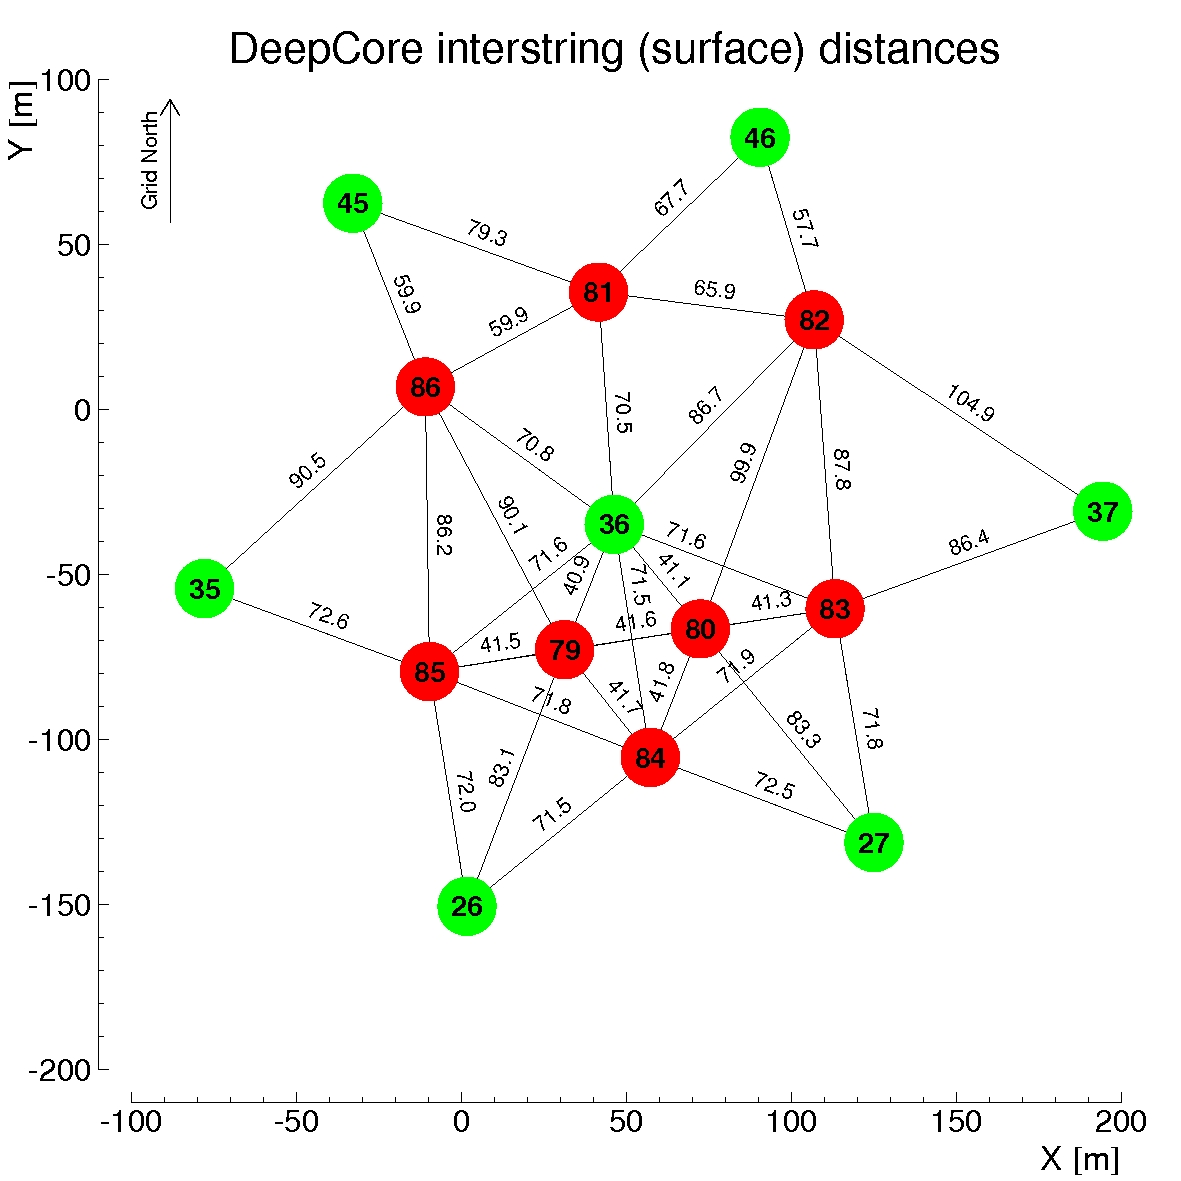
\includegraphics{figures/icecube_deepcore/deepcore_surface_distances.jpg}
    \caption[DeepCore string spacing]{Horizontal positions and distances between DeepCore strings. Red strings are instrumented more densely (vertically) and partially have higher quantum efficiency (HQE) DOMs.}
    \labfig{deepcore_distances}
\end{figure}

To investigate some idealistic double cascade event scenarios, two samples are produced for straight up-going events that are centered on a string and horizontal events located inside DeepCore.

\begin{table}
    \small
        \begin{tabular}{ llll }
        \hline\hline
        \textbf{Sample} & \textbf{Variable} & \textbf{Distribution} & \textbf{Range/Value} \\
        \hline\hline
        \multicolumn{2}{l}{Up-going} && \\
        \hline
        & energy & uniform & \SIrange{0.0}{60.0}{\gev} \\
        & zenith & fixed & \SI{180.0}{\degree} \\
        & azimuth & fixed & \SI{0.0}{\degree} \\
        & $x,y$ position & fixed & (41.6, 35.49)\,\si{\metre} \\
        & $z$ position & uniform & \SIrange{-480.0}{-180.0}{\metre} \\
        \hline
        \multicolumn{2}{l}{Horizontal} && \\ 
        \hline
        & energy & uniform & \SIrange{0.0}{60.0}{\gev} \\
        & zenith & fixed & \SI{90.0}{\degree} \\
        & azimuth & uniform & \SIrange{0.0}{360.0}{\degree} \\
        & $x,y$ position & uniform (circle) & $c$=(46.29, -34.88)\,\si{\metre}, $r$=\SI{150.0}{\metre} \\
        & $z$ position & fixed & \SI{-330.0}{\metre} \\
        \hline
        \end{tabular}
    \caption[Simplified model independent simulation sampling distributions]{Generation level sampling distributions and ranges/values of up-going and horizontal model independent simulation.}
    \labtab{hnl_simplified_sampling_distributions}
\end{table}

The first sample is used to investigate one of the most promising scenarios to detect a double cascade, where both cascade centers are located on a DeepCore string (namely string 81) and the directions are directly up-going. The horizontal positions and distances of all DeepCore fiducial volume strings are shown in \reffig{deepcore_distances} and string 81 is at a medium distance of $\sim\SI{70}{\metre}$ to its neighboring strings. As already mentioned in \refsec{deepcore}, DeepCore strings have higher quantum efficiency DOMs and a denser vertical spacing, making them better to detect low energetic events that produce little light. To produce the events, the $x,y$ position of the cascades is fixed to the center of string 81 while the $z$ positions are each sampled uniformly along the axis of the string. Note here that this will therefore not produce a uniform length distribution between the cascades. The positions are defined in the IceCube coordinate system that was already introduced in \refsec{icecube}. The energies are sampled uniformly between \SIrange[range-phrase={~and~}]{0.0}{60.0}{\gev}. The specific sampling distributions/values for the cascades are listed in \reftab{hnl_simplified_sampling_distributions}. The order of the cascades is chosen such that the lower one is first ($t_0=\SI{0.0}{\nano\second}$) and the upper one is second ($t_1=L/c$), assuming the speed of light $c$ as speed of the heavy mass state, traveling between the two cascades.
% The generation level distributions of the up-going sample are shown in \reffig{upgoing_string81_gen_distris}.

\begin{figure*}[h]
    \centering
    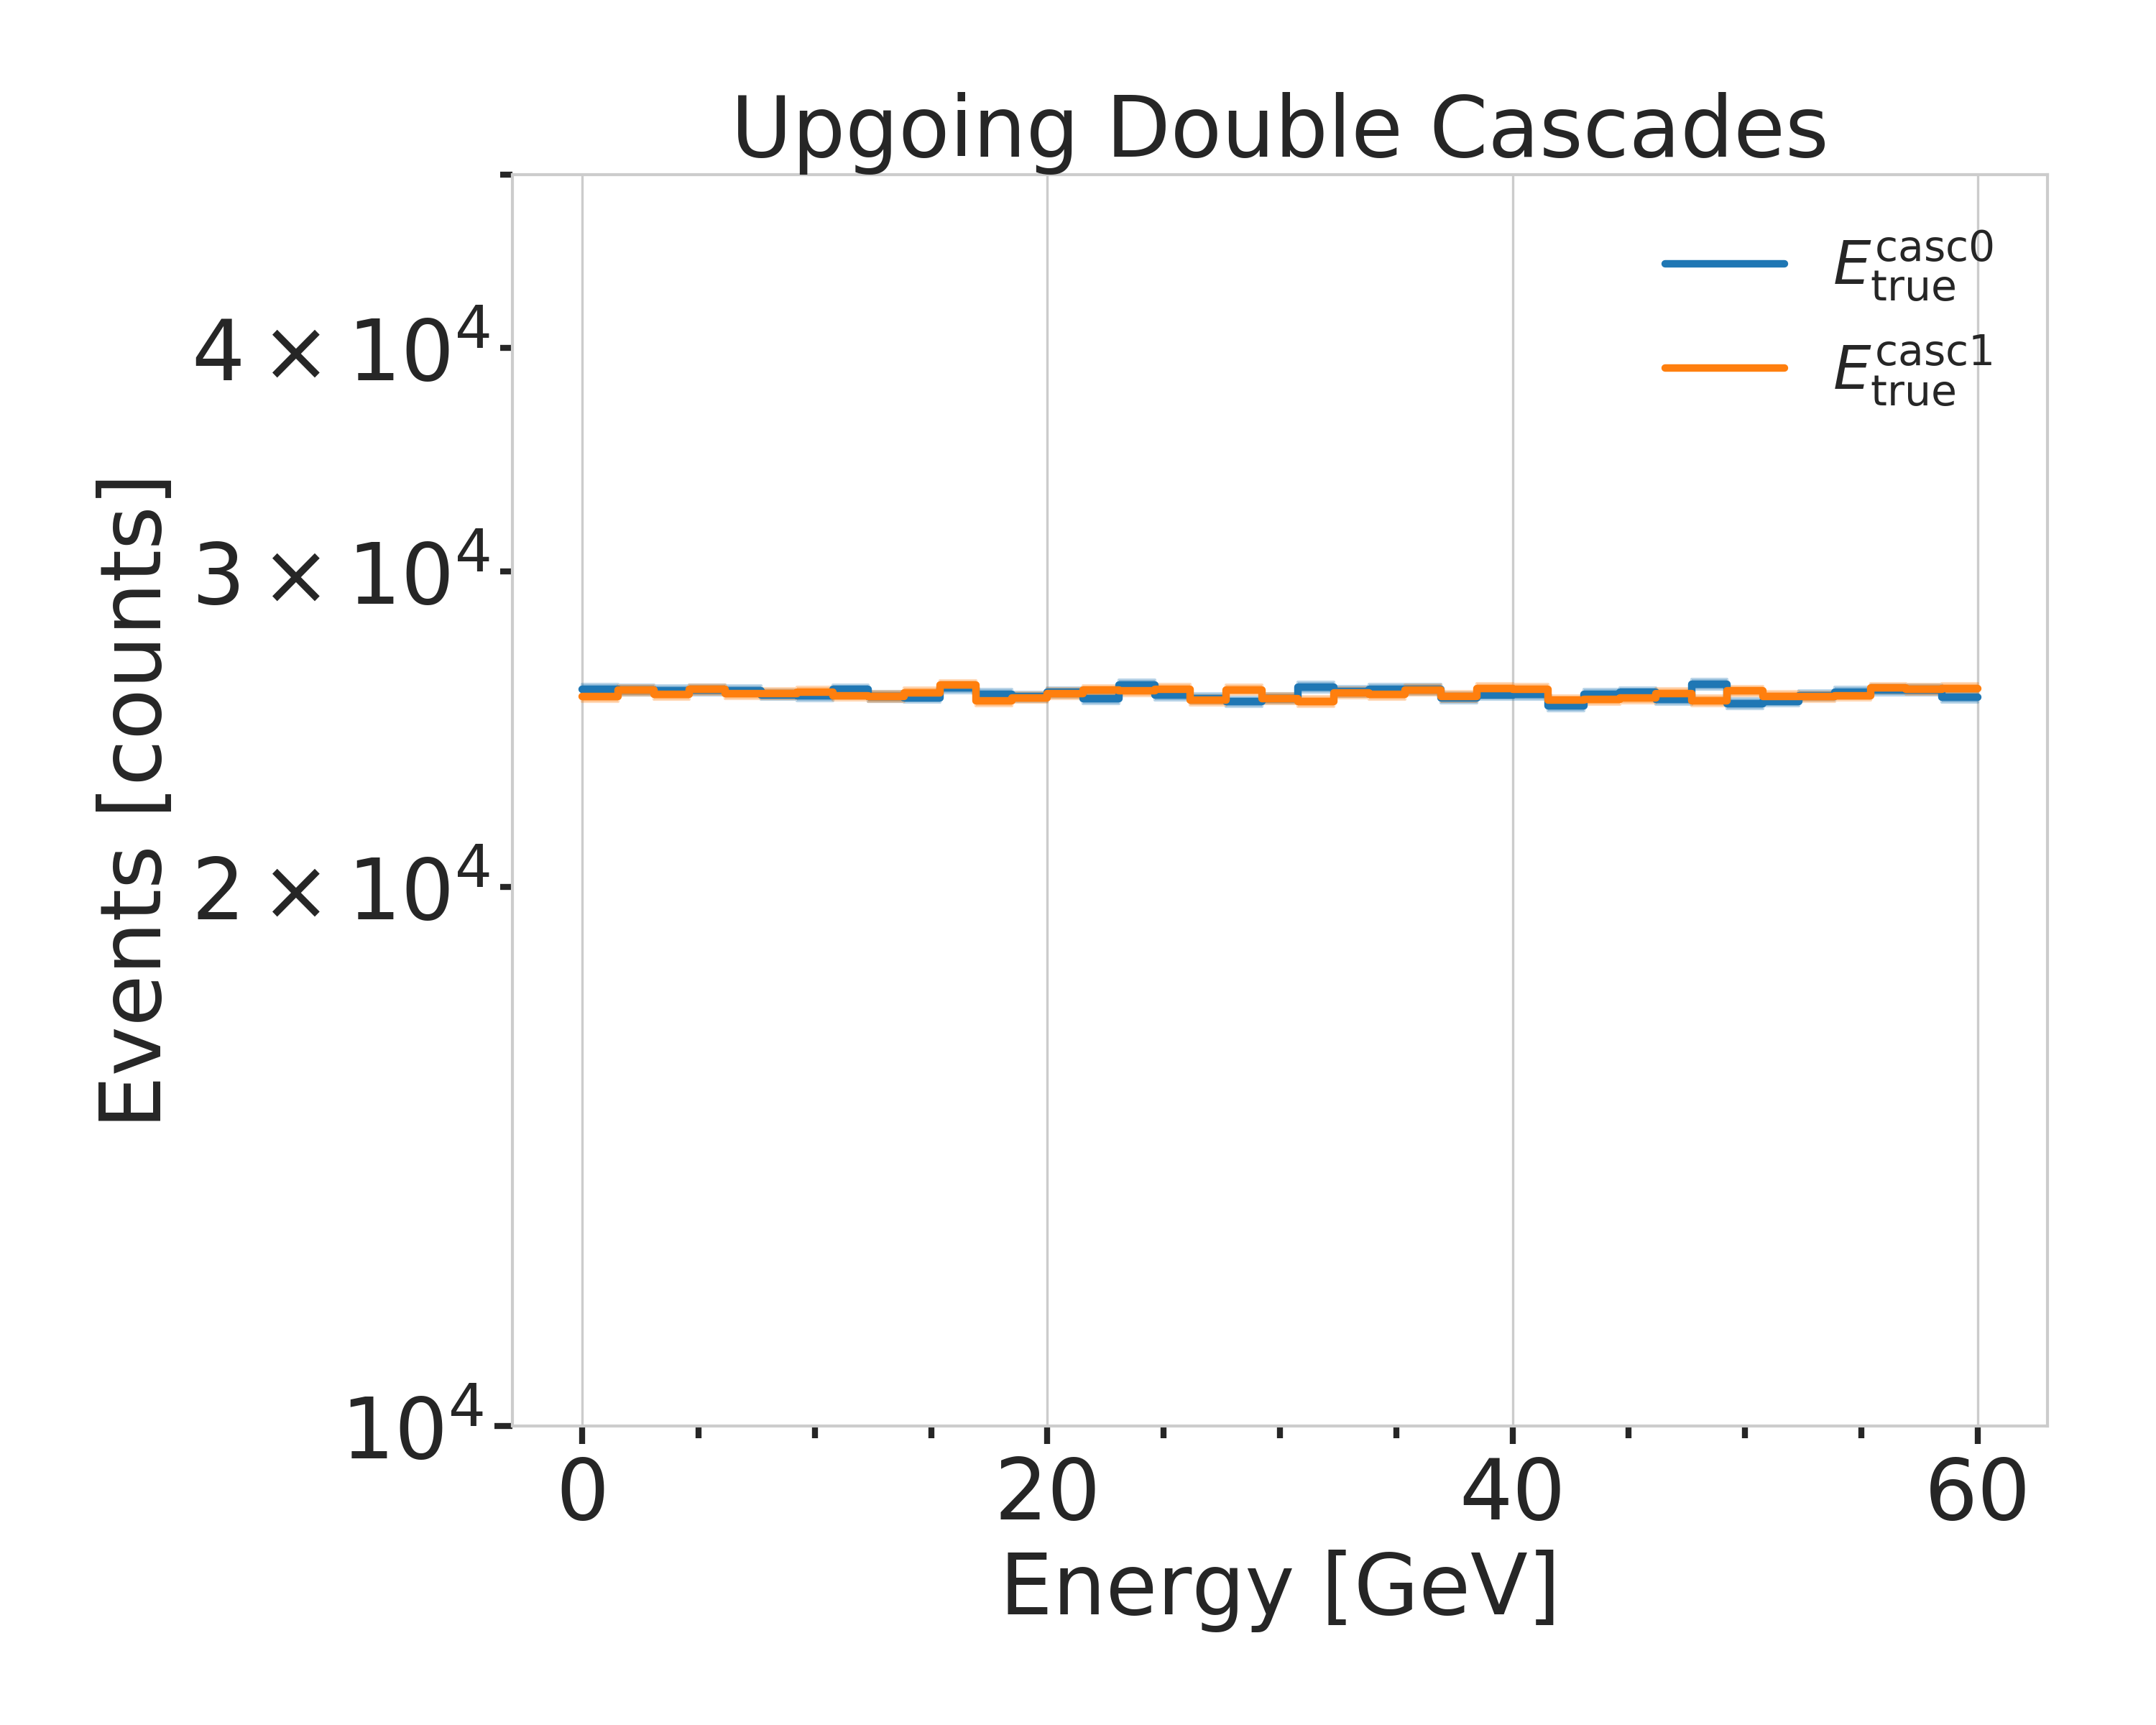
\includegraphics[width=.49\linewidth]{figures/model_independent_simulation/gen_level/1_d_distr_energies_clipped.png}
    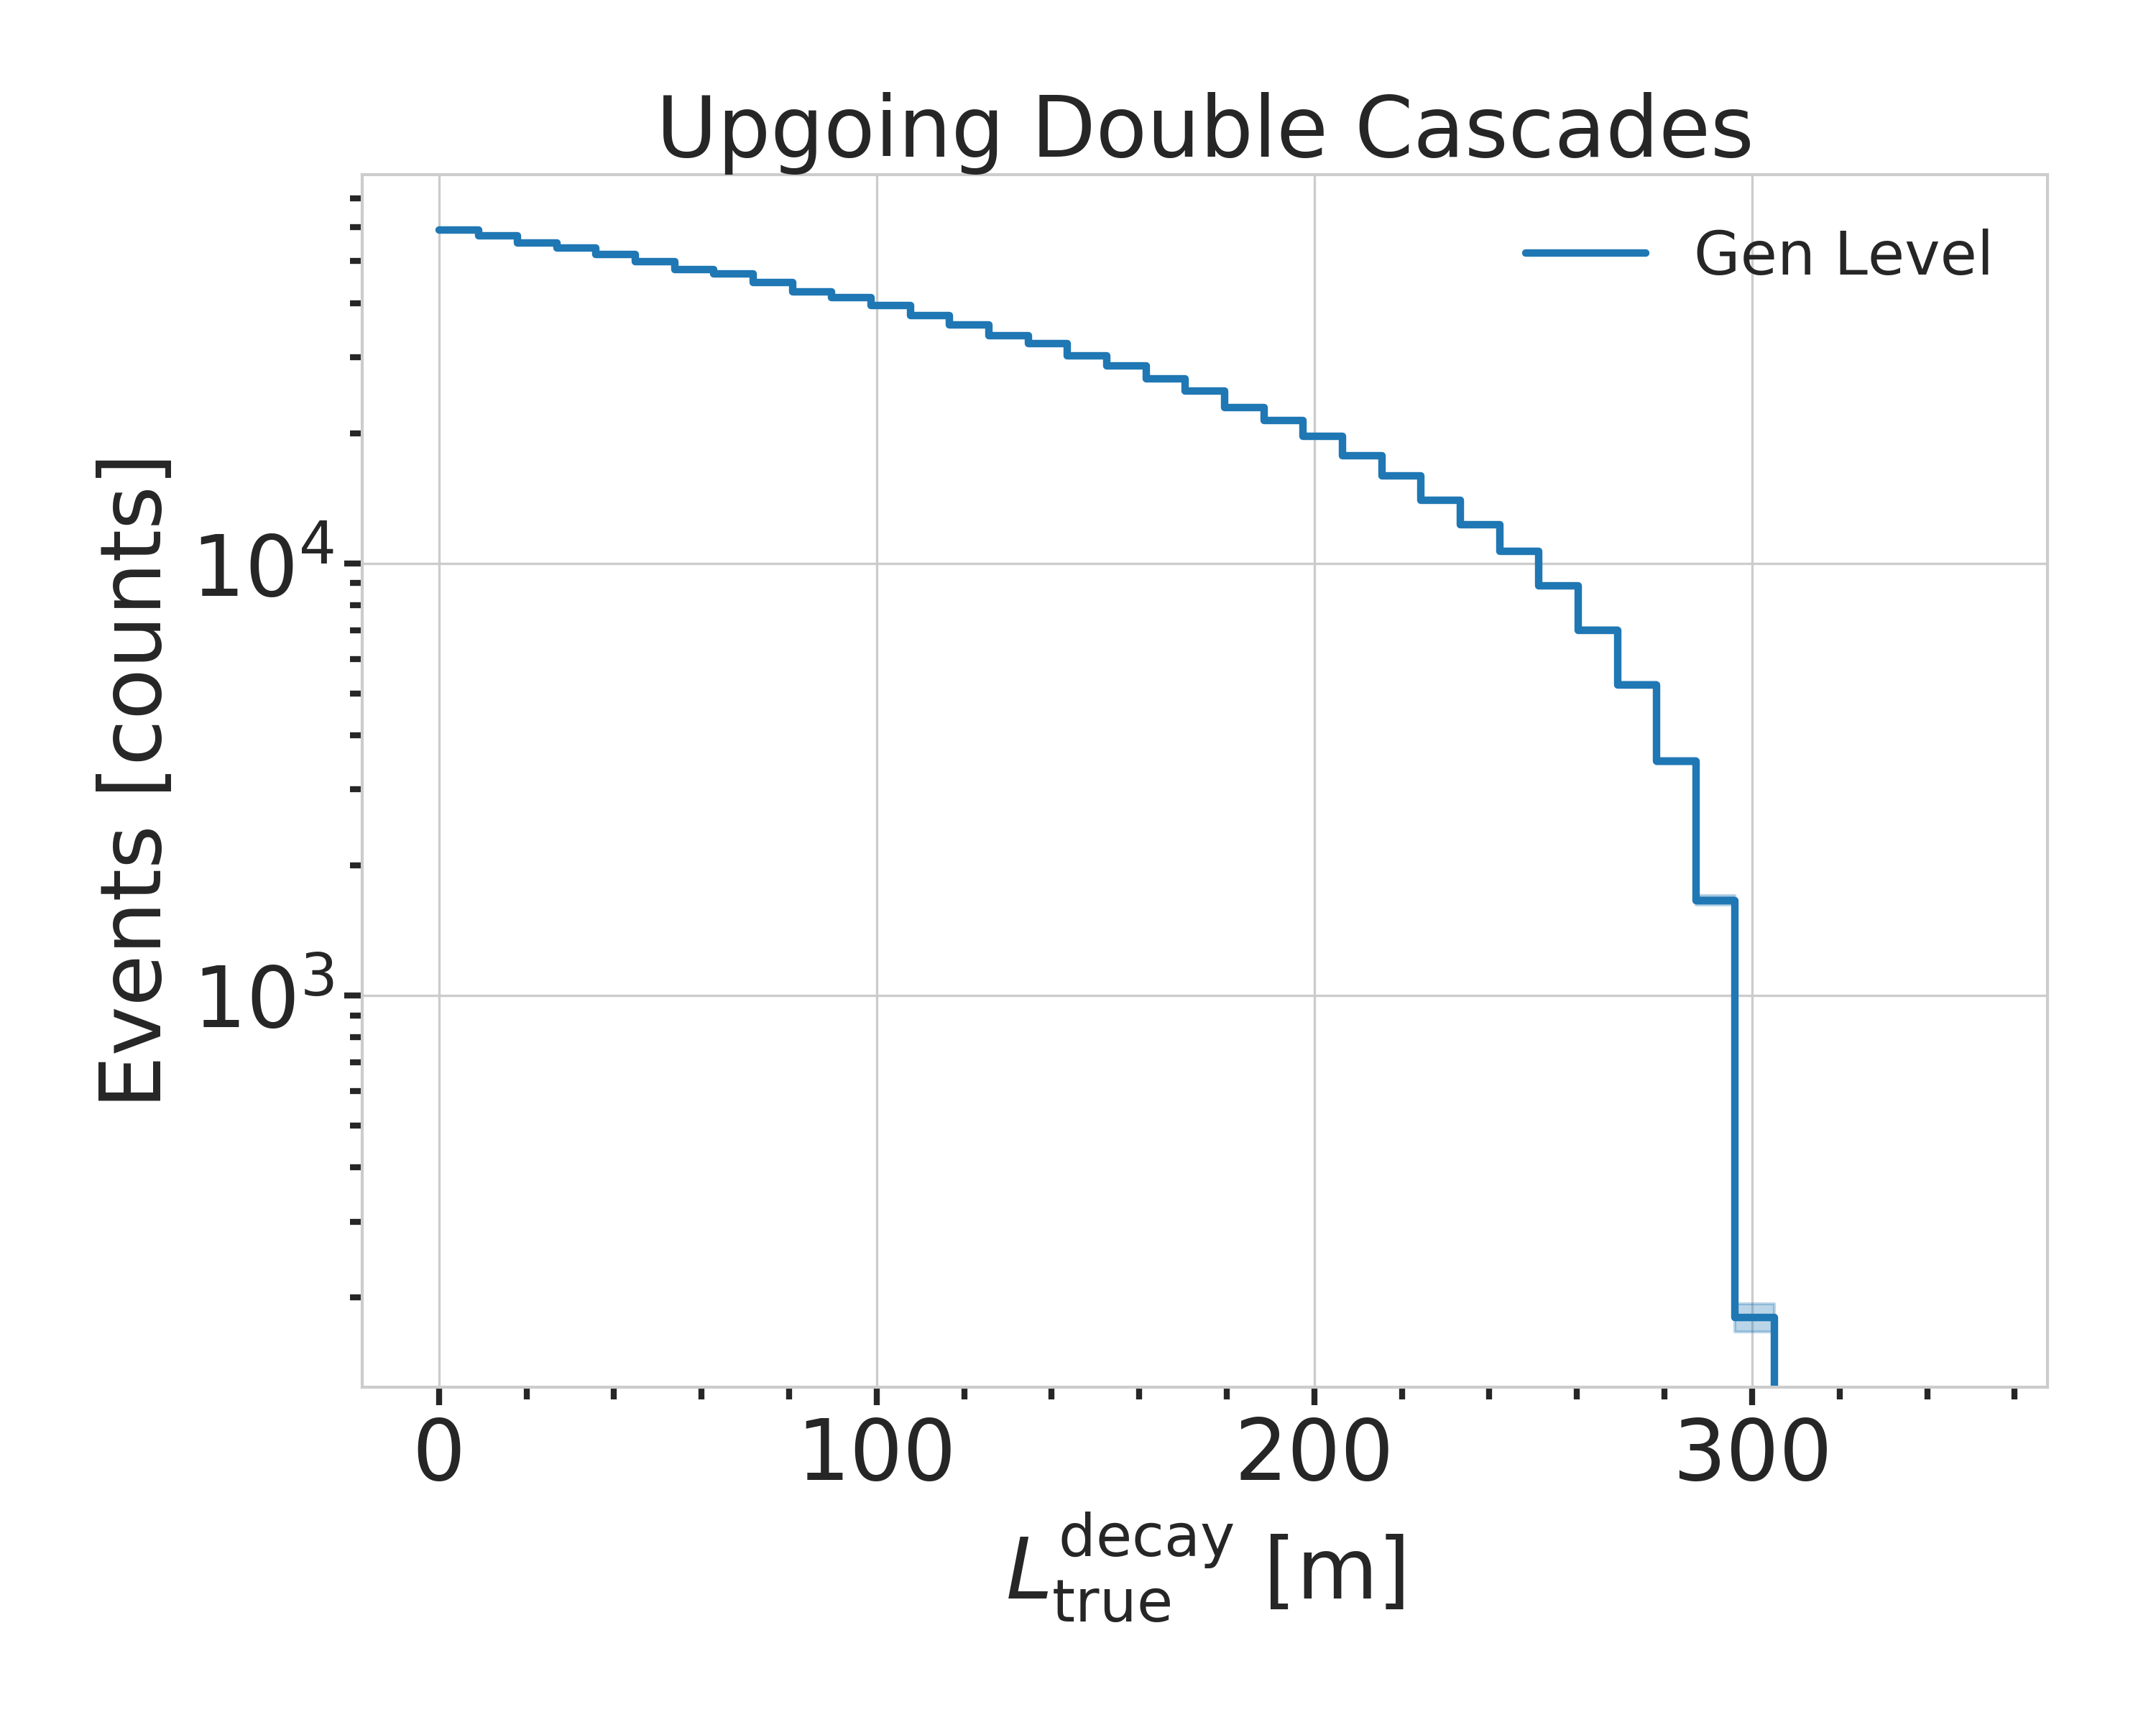
\includegraphics[width=.49\linewidth]{figures/model_independent_simulation/gen_level/1_d_distr_true_decay_length_clipped.png}
    \caption[Simplified model independent simulation generation level distributions]{Generation level distributions of the simplistic simulation samples. Cascade and total energies (left) and decay lengths (right) of both samples are shown.}
    \labfig{simplified_gen_distris}
\end{figure*}

\todo{Re-make plot with all energies (cascades and total, both samples (they are the same))}
\todo{Re-make plot with all decay lengths (both samples)}

The second sample is used to investigate the reconstruction performance for horizontal events, where the spacing between DOMs is much larger. The cascades are placed uniformly on a circle centered in DeepCore. The direction is always horizontal and azimuth is defined by the connecting vector of both cascade positions. The energies are again sampled uniformly between \SIrange[range-phrase={~and~}]{0.0}{60.0}{\gev} and the detailed sampling distributions/values are also listed in \reftab{hnl_simplified_sampling_distributions}. Some examples of the generation level distributions of the simplified samples are shown in \reffig{simplified_gen_distris}\todo{describe why these are shown to highlight some key aspect (uniformity in both energies to sample the whole space, decay length as a result of the z sampling etc..), also add this shortly to the caption}, while further distributions can be found in \reffig{simplified_gen_distris_appendix}.
% The variables that are uniformly sampled or fixed to a certain value are not presented.


\subsection{Realistic Sample}

To thoroughly investigate the potential of IceCube DeepCore to detect double cascade events, a more realistic simulation sample is produced that aims to be as close as possible to the expected signal simulation explained in \refsec{model_specific_simulation}, while still allowing additional freedom to control the double cascade kinematics. For this purpose the total energy is sampled from an $E^{-2}$ power law, mimicking the energy spectrum of the primary neutrinos as stated in \refsec{neutrino_generation}.
% Although in the realistic process described in \refsec{model_specific_simulation} the energy is distributed in a more complex way into the two cascades and secondary particles, it is a good approximation to simply
The total energy is divided into two parts, by assigning a fraction between \SIrange[range-phrase={~and~}]{0}{100}{\percent} to one cascade and the remaining part to the other cascade. This is a generic approximation of the realistic process described in \refsec{model_specific_simulation}, and chosen such that the whole sample covers various cases of energy distributions between the two cascades. To efficiently generate events in a way that produces distributions similar to what would be observed with DeepCore, one of the cascade positions is sampled inside the DeepCore volume by choosing its coordinates uniformly on a cylinder that is centered in DeepCore. This is similar to a trigger condition of one cascade always being inside the DeepCore fiducial volume. By choosing the direction of the event by sampling zenith and azimuth uniformly between \SIrange[range-phrase={~and~}]{70}{180}{\degree} and \SIrange[range-phrase={~and~}]{0}{360}{\degree}, respectively, the position of the other cascade can be inferred for a given decay length, assuming a travel speed of $c$, and choosing whether the cascade position that was sampled is the first cascade or the second with a \SI{50}{\percent} chance. The decay length is sampled from an exponential distribution, as expected for a decaying heavy mass state.
% Based on the direction and the decay length, the position of the other cascade is found, assuming a travel speed of $c$ and randomly choosing whether the cascade position that was sampled is the first cascade or the second and then assigning the other cascade position accordingly.
The sampling distributions/values are listed in \reftab{hnl_realistic_sample_sampling_distributions}. Example distributions of the generation level variables are shown in \reffig{realistic_gen_distris}\todo{again, describe what is shown and why this is interesting (e.g. energy distribution between the cascades, realistic exponential decay length distribtuion..) also add this to the captions shortly}, while further distributions can be found in \reffig{realistic_gen_distris_appendix}.

\begin{table}
    \small
        \begin{tabular}{ llll }
        \hline\hline
        \textbf{Variable} & \textbf{Distribution} & \textbf{Range/Value} \\
        \hline\hline
        energy (total) & power law $E^{-2}$ & \SIrange{1}{1000}{\gev} \\
        decay length & exponential e$^{-0.01L}$ & \SIrange{0}{1000}{\metre} \\
        zenith & uniform & \SIrange{70}{180}{\degree} \\
        azimuth & uniform & \SIrange{0}{360}{\degree} \\
        $x,y$ (one cascade) & uniform (circle) & $c$=(46.29, -34.88)\,\si{\metre}, $r$=\SI{150}{\metre} \\
        $z$ (one cascade) & uniform & \SIrange{-480.0}{-180.0}{\metre}\\
        \hline
        \end{tabular}
        \caption[Realistic model independent simulation sampling distributions]{Generation level sampling distributions and ranges/values of the realistic model independent simulation.}
    \labtab{hnl_realistic_sample_sampling_distributions}
\end{table}

\begin{figure*}
        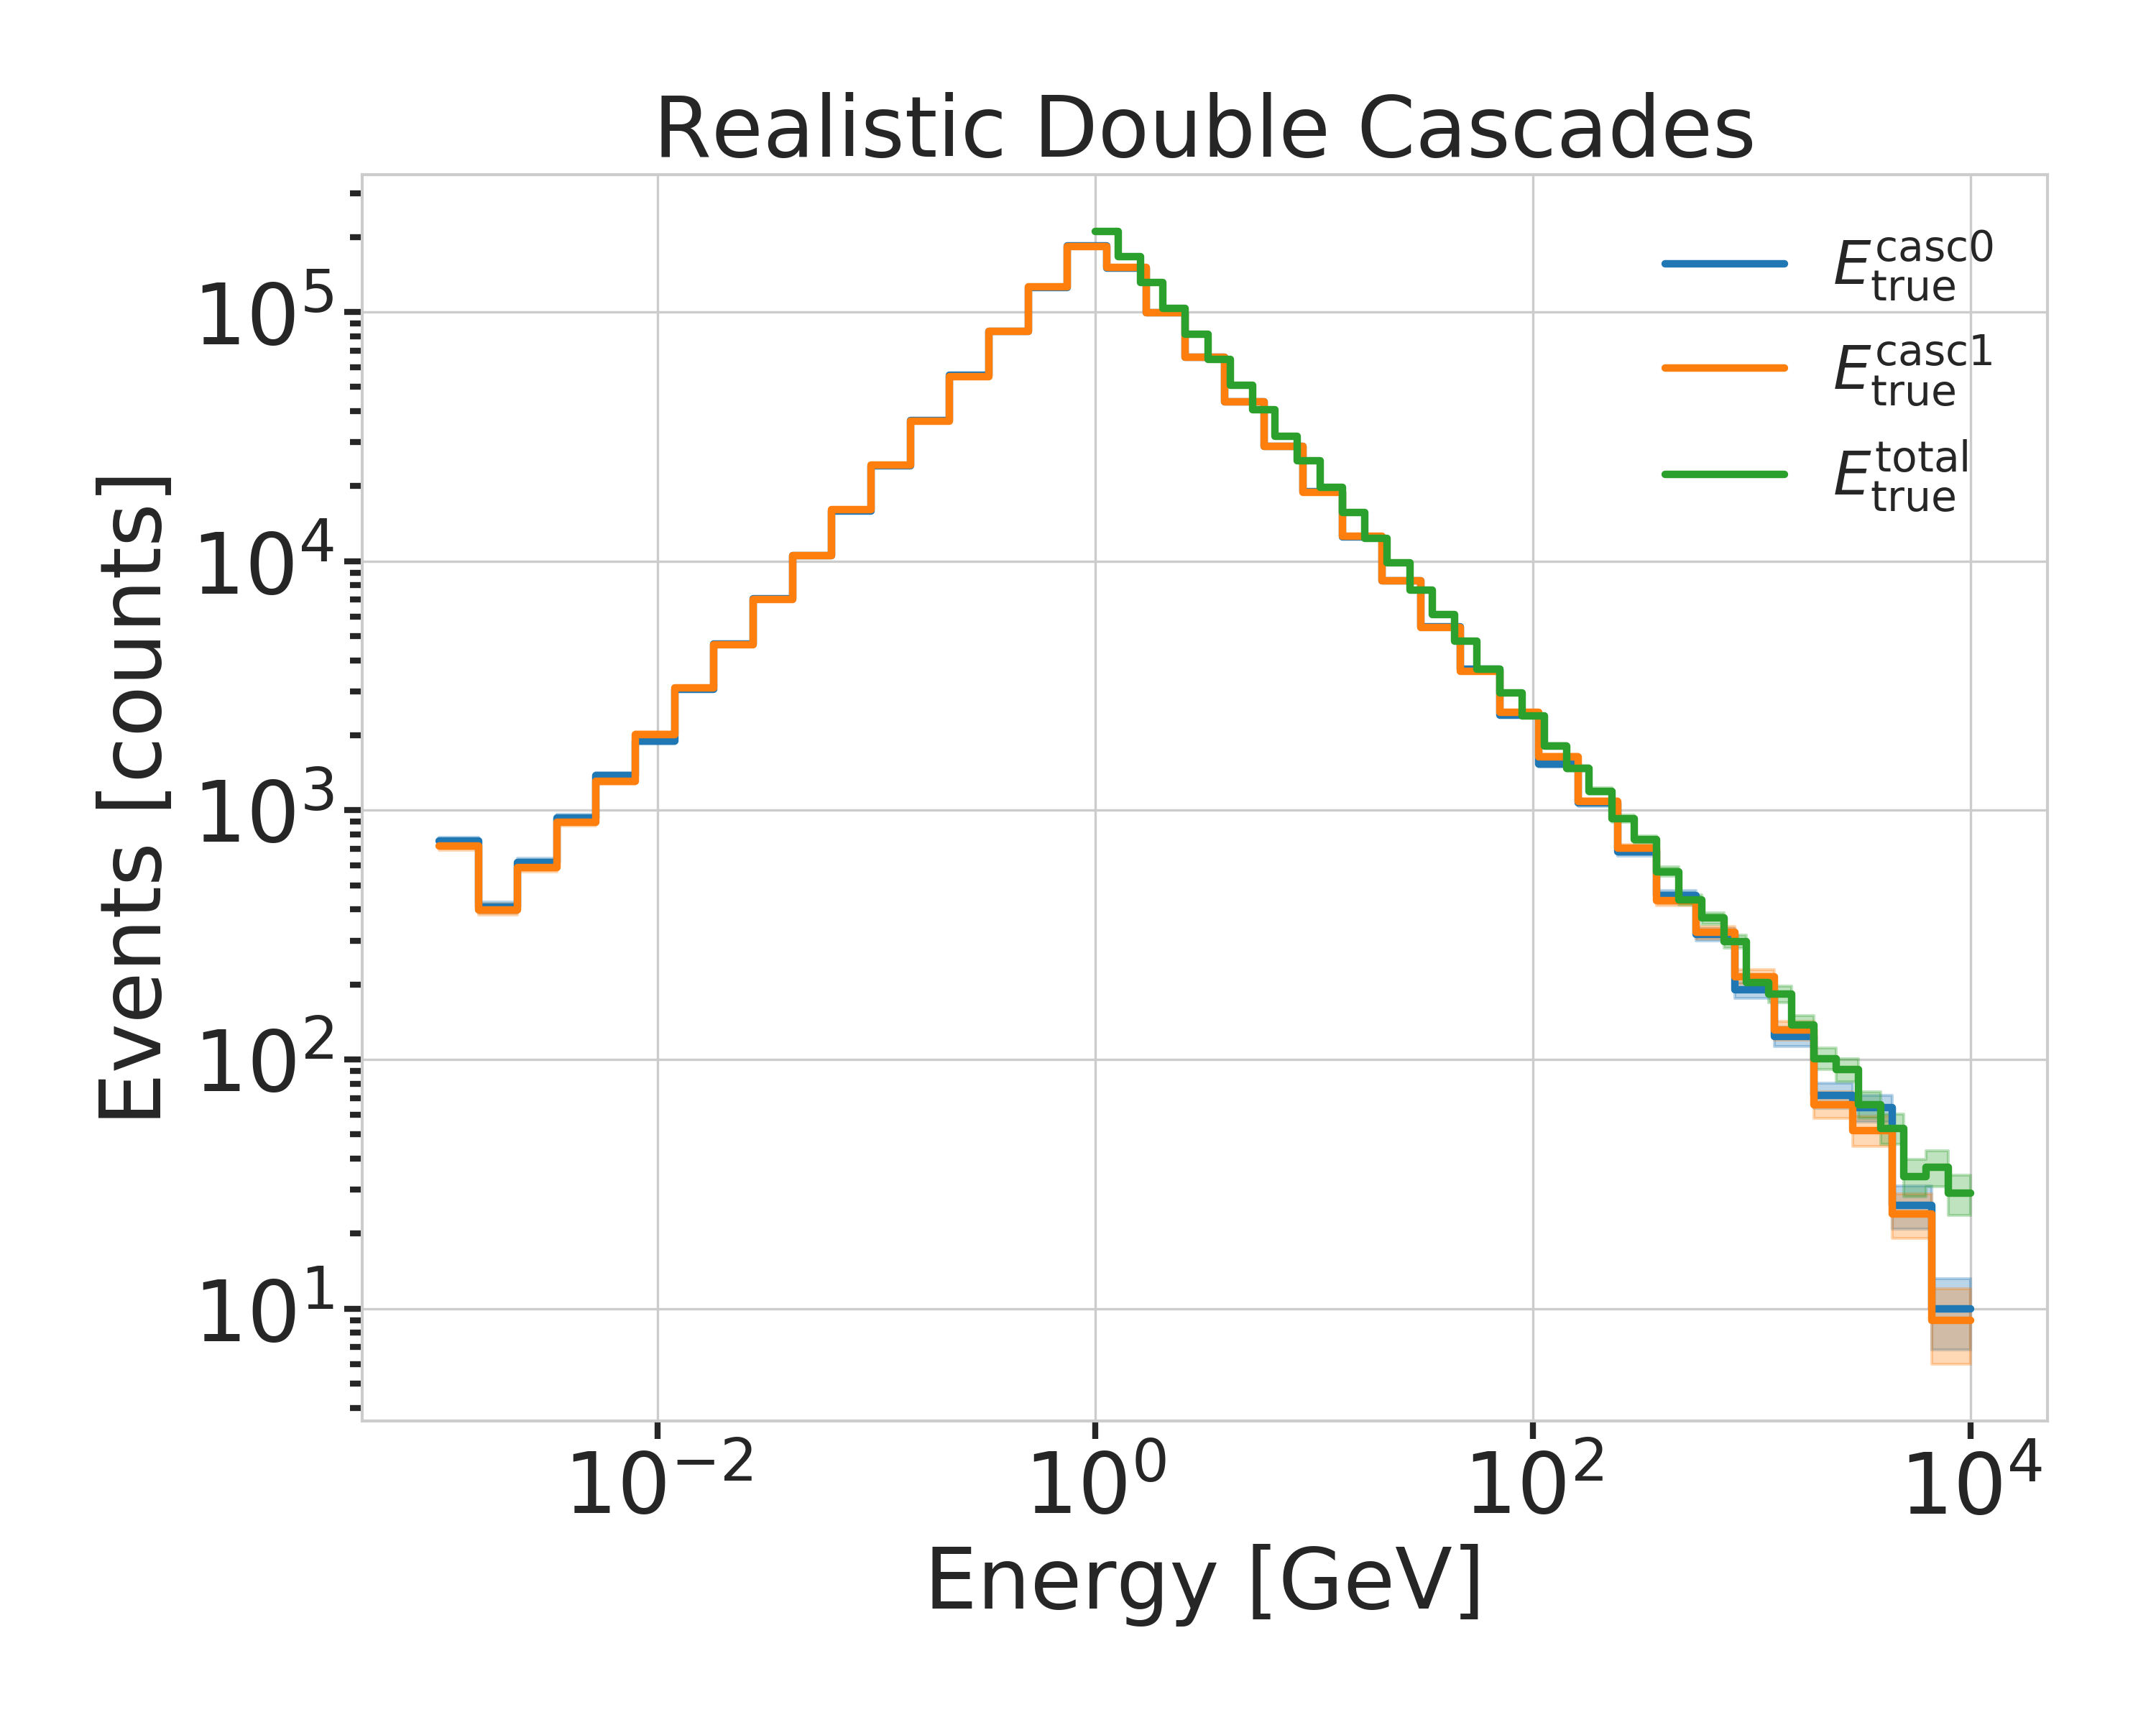
\includegraphics[width=.49\linewidth]{figures/model_independent_simulation/gen_level/194603_gen_level_1_d_distr_all_energies_clipped.png}
        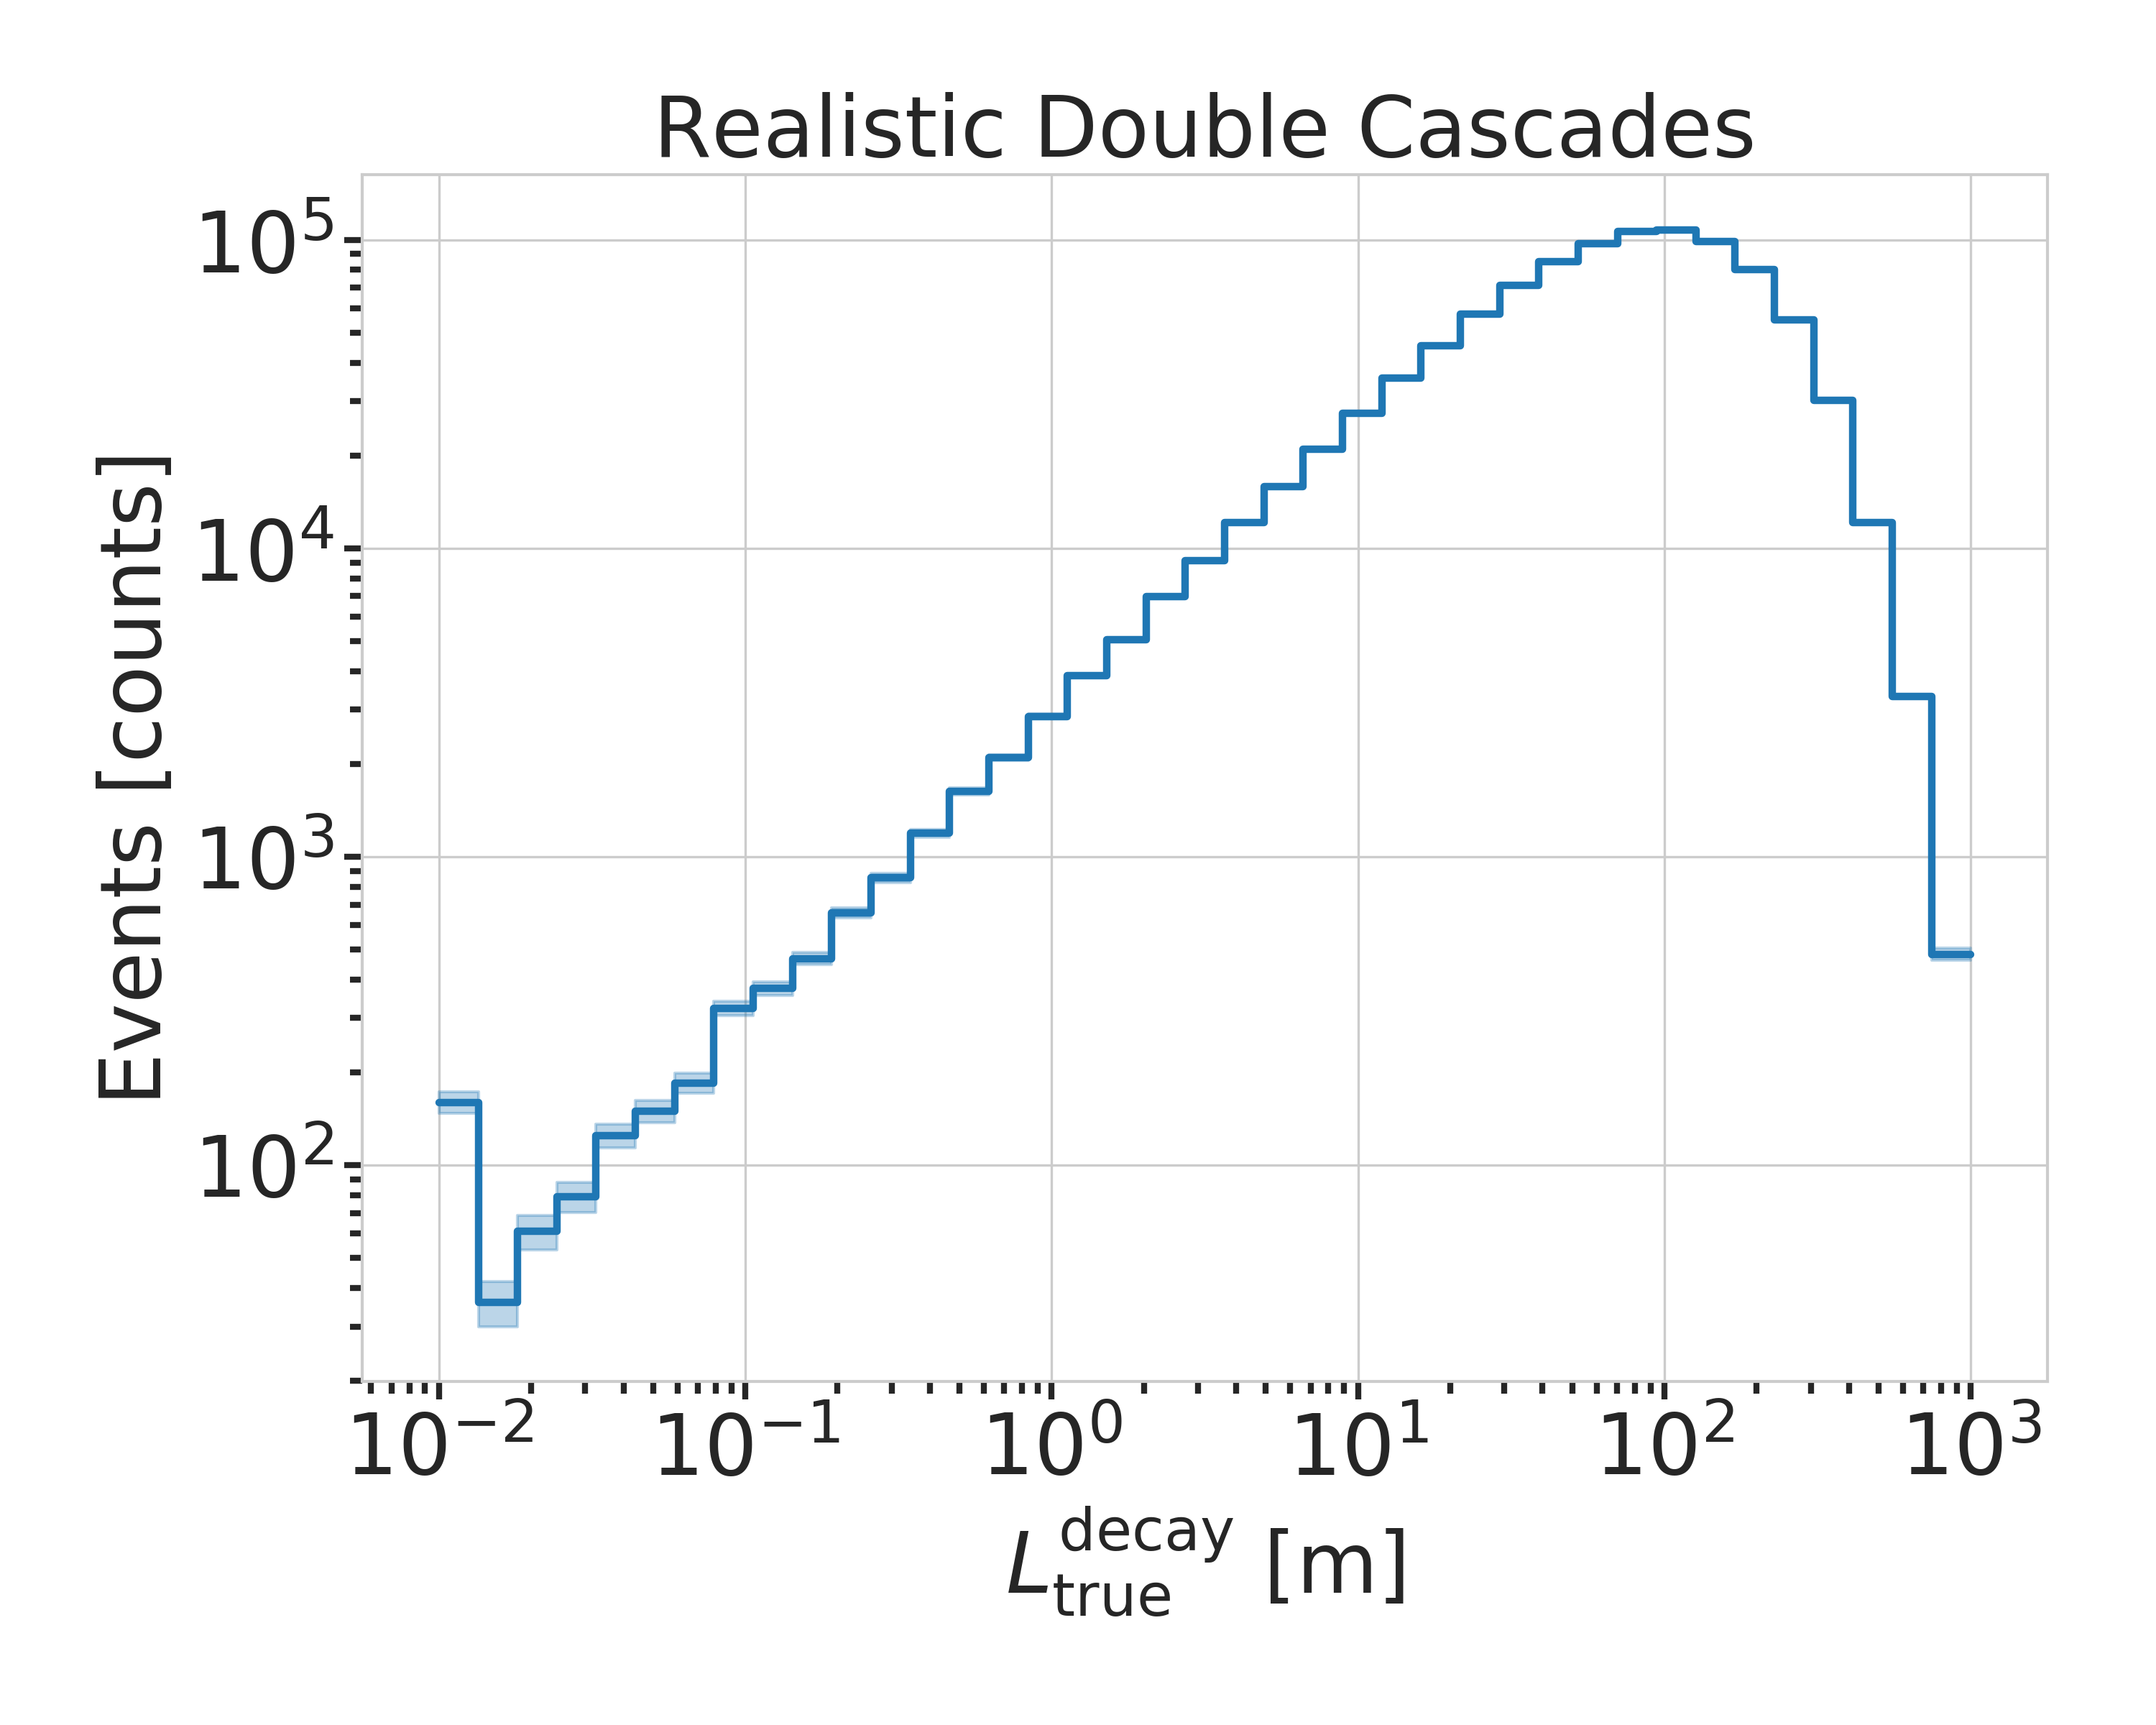
\includegraphics[width=.49\linewidth]{figures/model_independent_simulation/gen_level/194603_gen_level_1_d_distr_true_decay_length_clipped.png}
    \caption[Realistic model independent simulation generation level distributions]{Generation level distributions of the simplistic realistic sample. Shown are the cascade and total energies (left) and decay lengths (right).}
    \labfig{realistic_gen_distris}
\end{figure*}


\section{Model Dependent Simulation} \labsec{model_specific_simulation}

To estimate the HNL event expectation in IceCube DeepCore, depending on the specific model parameters, a generator was developed that is based on the HNL theory introduced in \refsec{hnl_theory}. For this work, only the interaction with the $\tau$-sector was taken into account ($|U_{\alpha4}^2|=0$, $\alpha=e,\mu$), which reduces the physics parameters of interest and relevent for the simulation to the fourth heavy lepton mass, $m_4$, and the mixing, $|U_{\tau4}^2|$. The generator uses a customized \textit{\textsc{LeptonInjector} (LI)} version to create the events and \textit{\textsc{LeptonWeighter} (LW)} to weight them \sidecite{IceCube:2020tcq}. The modified LI and the essential components needed for the HNL simulation are described in the next sections, followed by the description of the weighting scheme and the sampling distributions chosen for the simulation generation.


\subsection{Custom LeptonInjector} \labsec{custom_leptoninjector}

In its standard version, the LI generator produces neutrino interactions by injecting a lepton and a hadronic cascade at the interaction vertex of the neutrino, where the lepton is the charged (neutral) particle produced in a CC (NC) interaction and the cascade is the hadronic cascade from the breaking nucleus. The hadronic cascade is stored as a specific object of type \textit{Hadrons}, which triggers the correct simulation of the shower development in the following simulation steps, identical to what will be described for SM neutrino simulation on \refsec{neutrino_generation}. The main differences to an EM cascade is that part of the energy will not be observed, because it goes into neutral particles, and that the spatial development of the shower is different. Both objects are injected with the same $(x,y,z,t)$ coordinates and the kinematics are sampled from the differential and total cross-sections that are one of the inputs to LI.

\todo{JVS:
    consider remaking figures at the native size so type size is consistent. Also, consider making the legend box semi-transparent so the lines do not obscure the text and markers.
}

\begin{figure}[h]
    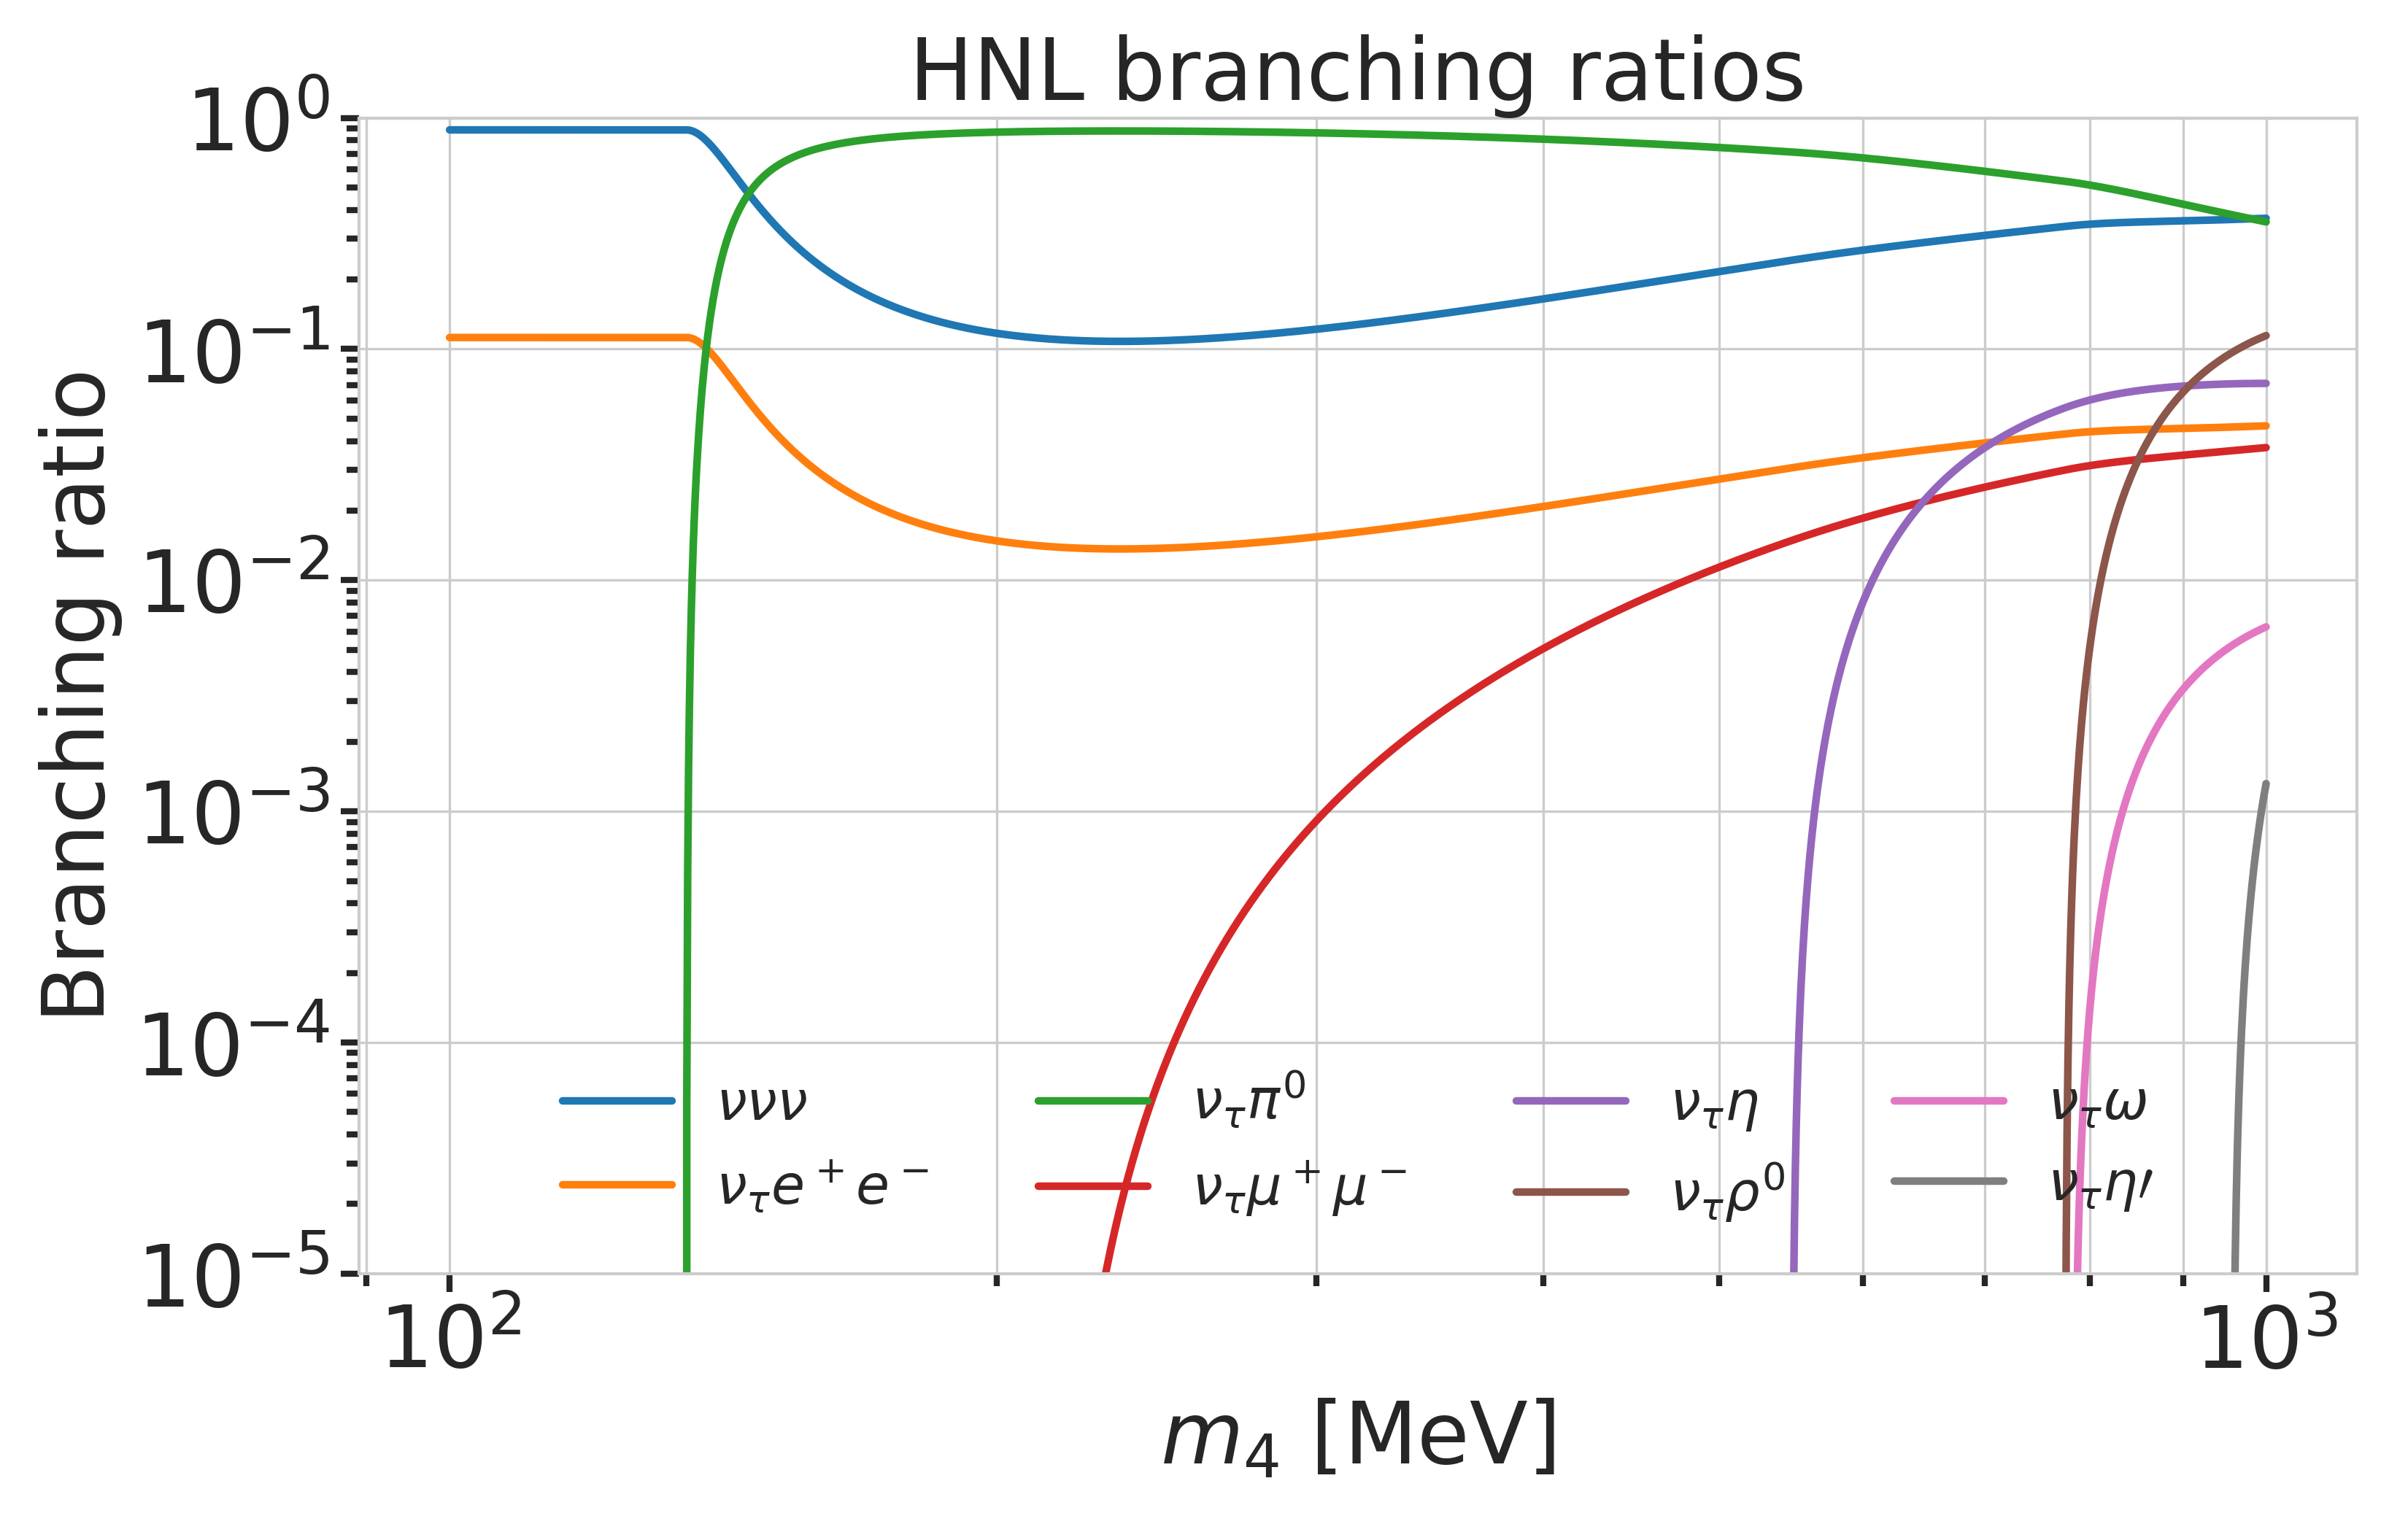
\includegraphics{hnl_simulation/decay_theory/branching_ratios_log_up_to_1.0_GeV.png}
    \caption[HNL branching ratios]{Branching ratios of the HNL within the mass range considered in this work, only considering $|U_{\tau4}^2| \neq 0$, calculated based on the results from \cite{Coloma:2020lgy}.}
    \labfig{hnl_branching_ratios}
\end{figure}

In the modified version, the SM lepton at the interaction vertex is replaced by the new HNL particle, where the interaction cross-sections are replaced by custom, mass dependent HNL cross-sections. The HNL is forced to decay after a chosen distance\sidenote{The explicit sampling distributions and ranges can be found in \refsec{hnl_sampling_distributions}.} to produce secondary SM particles, where the decay mode is chosen with a probability given by the mass dependent branching ratios from the kinematically accessible decay modes shown in \reffig{hnl_branching_ratios}. The cross-section and decay width calculations were implemented for this purpose and will be explained in more detail in the following. Another needed addition to LI is that the decay products of the HNL are also added to the list of MC particles in each event. They are injected with the correctly displaced position and delayed time from the interaction vertex, given the HNL decay length. These HNL daughter particles form the second cascade, not as a single hadronic cascade object, but as the explicit particles forming the shower. The kinematics of the two-body decays are computed analytically, while the three-body decay kinematics are calculated with \textsc{MadGraph} \sidecite{madgraph}, which will also be explained further below. Independent of the number of particles in the final state of the HNL decay, the kinematics are calculated/simulated at rest and then boosted along the HNL momentum. 

The injection is done using the LI \textit{volume mode}, for the injection of the primary particle on a cylindrical volume, adding \SI{50}{\percent} of the events with $\nu_\tau$ and the other half with $\bar{\nu}_\tau$ as primary particle types. The generator takes the custom double-differential/total cross-section splines described below and the parameters defining the sampling distributions as inputs.

% For each frame \textit{OneWeight} and a reference weight are also calculated and stored using the \href{https://github.com/LeanderFischer/LeptonInjector-HNL/blob/main/LeptonInjector/python/hnl_weighting.py}{weighting functions} and a baseline atmospheric $\nu_\tau$ flux + oscillation spline. The weight will later be calculated inside of the analysis framework \href{https://github.com/icecube/pisa}{PISA}, based on the input OneWeight. In addition to the i3 file itself, a LeptonInjector configuration file is written which stores the needed information to produce event weights using LeptonWeighter. Optionally the script can also produce an hdf5 file with the same name in the same location. This will store a fixed set of keys, extracted from the i3 file.


\subsubsection{Cross-Sections} \labsec{hnl_cross_sections}

\todo{Maybe decide if I want to handle git repo urls/references in a different way.. currently (without date+title) they look ugly in the margin, so I just state them as regular cites, but Cris gave me some other ideas on how to handle them.. (YELLOW)}

The cross-sections are calculated using the \textsc{NuXSSplMkr} \cite{xsecmaker} software, which is a tool to calculate neutrino cross-sections from \textit{parton distribution functions (PDFs)} and then fit to an N-dimensional tensor-product B-spline surface \sidecite{photospline} to produce the splines that can be read and used with LI/LW. The tool was modified to produce the custom HNL cross-sections, where the main modification to calculate the cross-sections for the $\nu_\tau$-NC interaction into the new heavy mass state, is the addition of a kinematic condition to ensure that there is sufficient energy to produce the heavy mass state. It is the same condition fulfilled for the CC case, where the outgoing charged lepton mass is non-zero. Following \sidecite{Levy:2004rk} (equation 7), the condition
\begin{equation}
    (1 + x \delta_N) h^2 - (x + \delta_{4}) h + x \delta_{4} \leq 0
    \;
    \labeq{hnl_kinematic_condition}
\end{equation}
is implemented for the NC case in the NuXSSplMkr code. Here
% write in equations: $\delta_{4}=\frac{m_4^2}{s-M^2}$, $\delta_{N}=\frac{M^2}{s-M^2}$, and $h \overset{\textit{def}}{=} xy + \delta_{4}$
\begin{align}
    \delta_{4} ={}& \frac{m_4^2}{s-M^2}
    \;, \\
    \delta_{N} ={}& \frac{M^2}{s-M^2}
    \;, \rm{and} \\
    h \overset{\textit{def}}{=}& xy + \delta_{4}
    \;,
    \labeq{hnl_kinematic_condition_variables}
\end{align}
with $x$ and $y$ being the Bjorken variables, $m_4$ and $M$ the mass of the heavy state and the target nucleon, respectively, and $s$ the center of mass energy squared. The custom version was made part of the open source NuXSSplMkr software and can thus be found in \cite{xsecmaker}. The result of this kinematic condition is that events cannot be produced for energy, $x$, $y$ combinations that don't have sufficient energy going into the outgoing, massive lepton. This results in a reduction of the cross-section towards lower energies, which scales with the assumed mass of the HNL. This effect can clearly be seen in \reffig{custom_hnl_cross_sections}.

\begin{figure*}[h]
    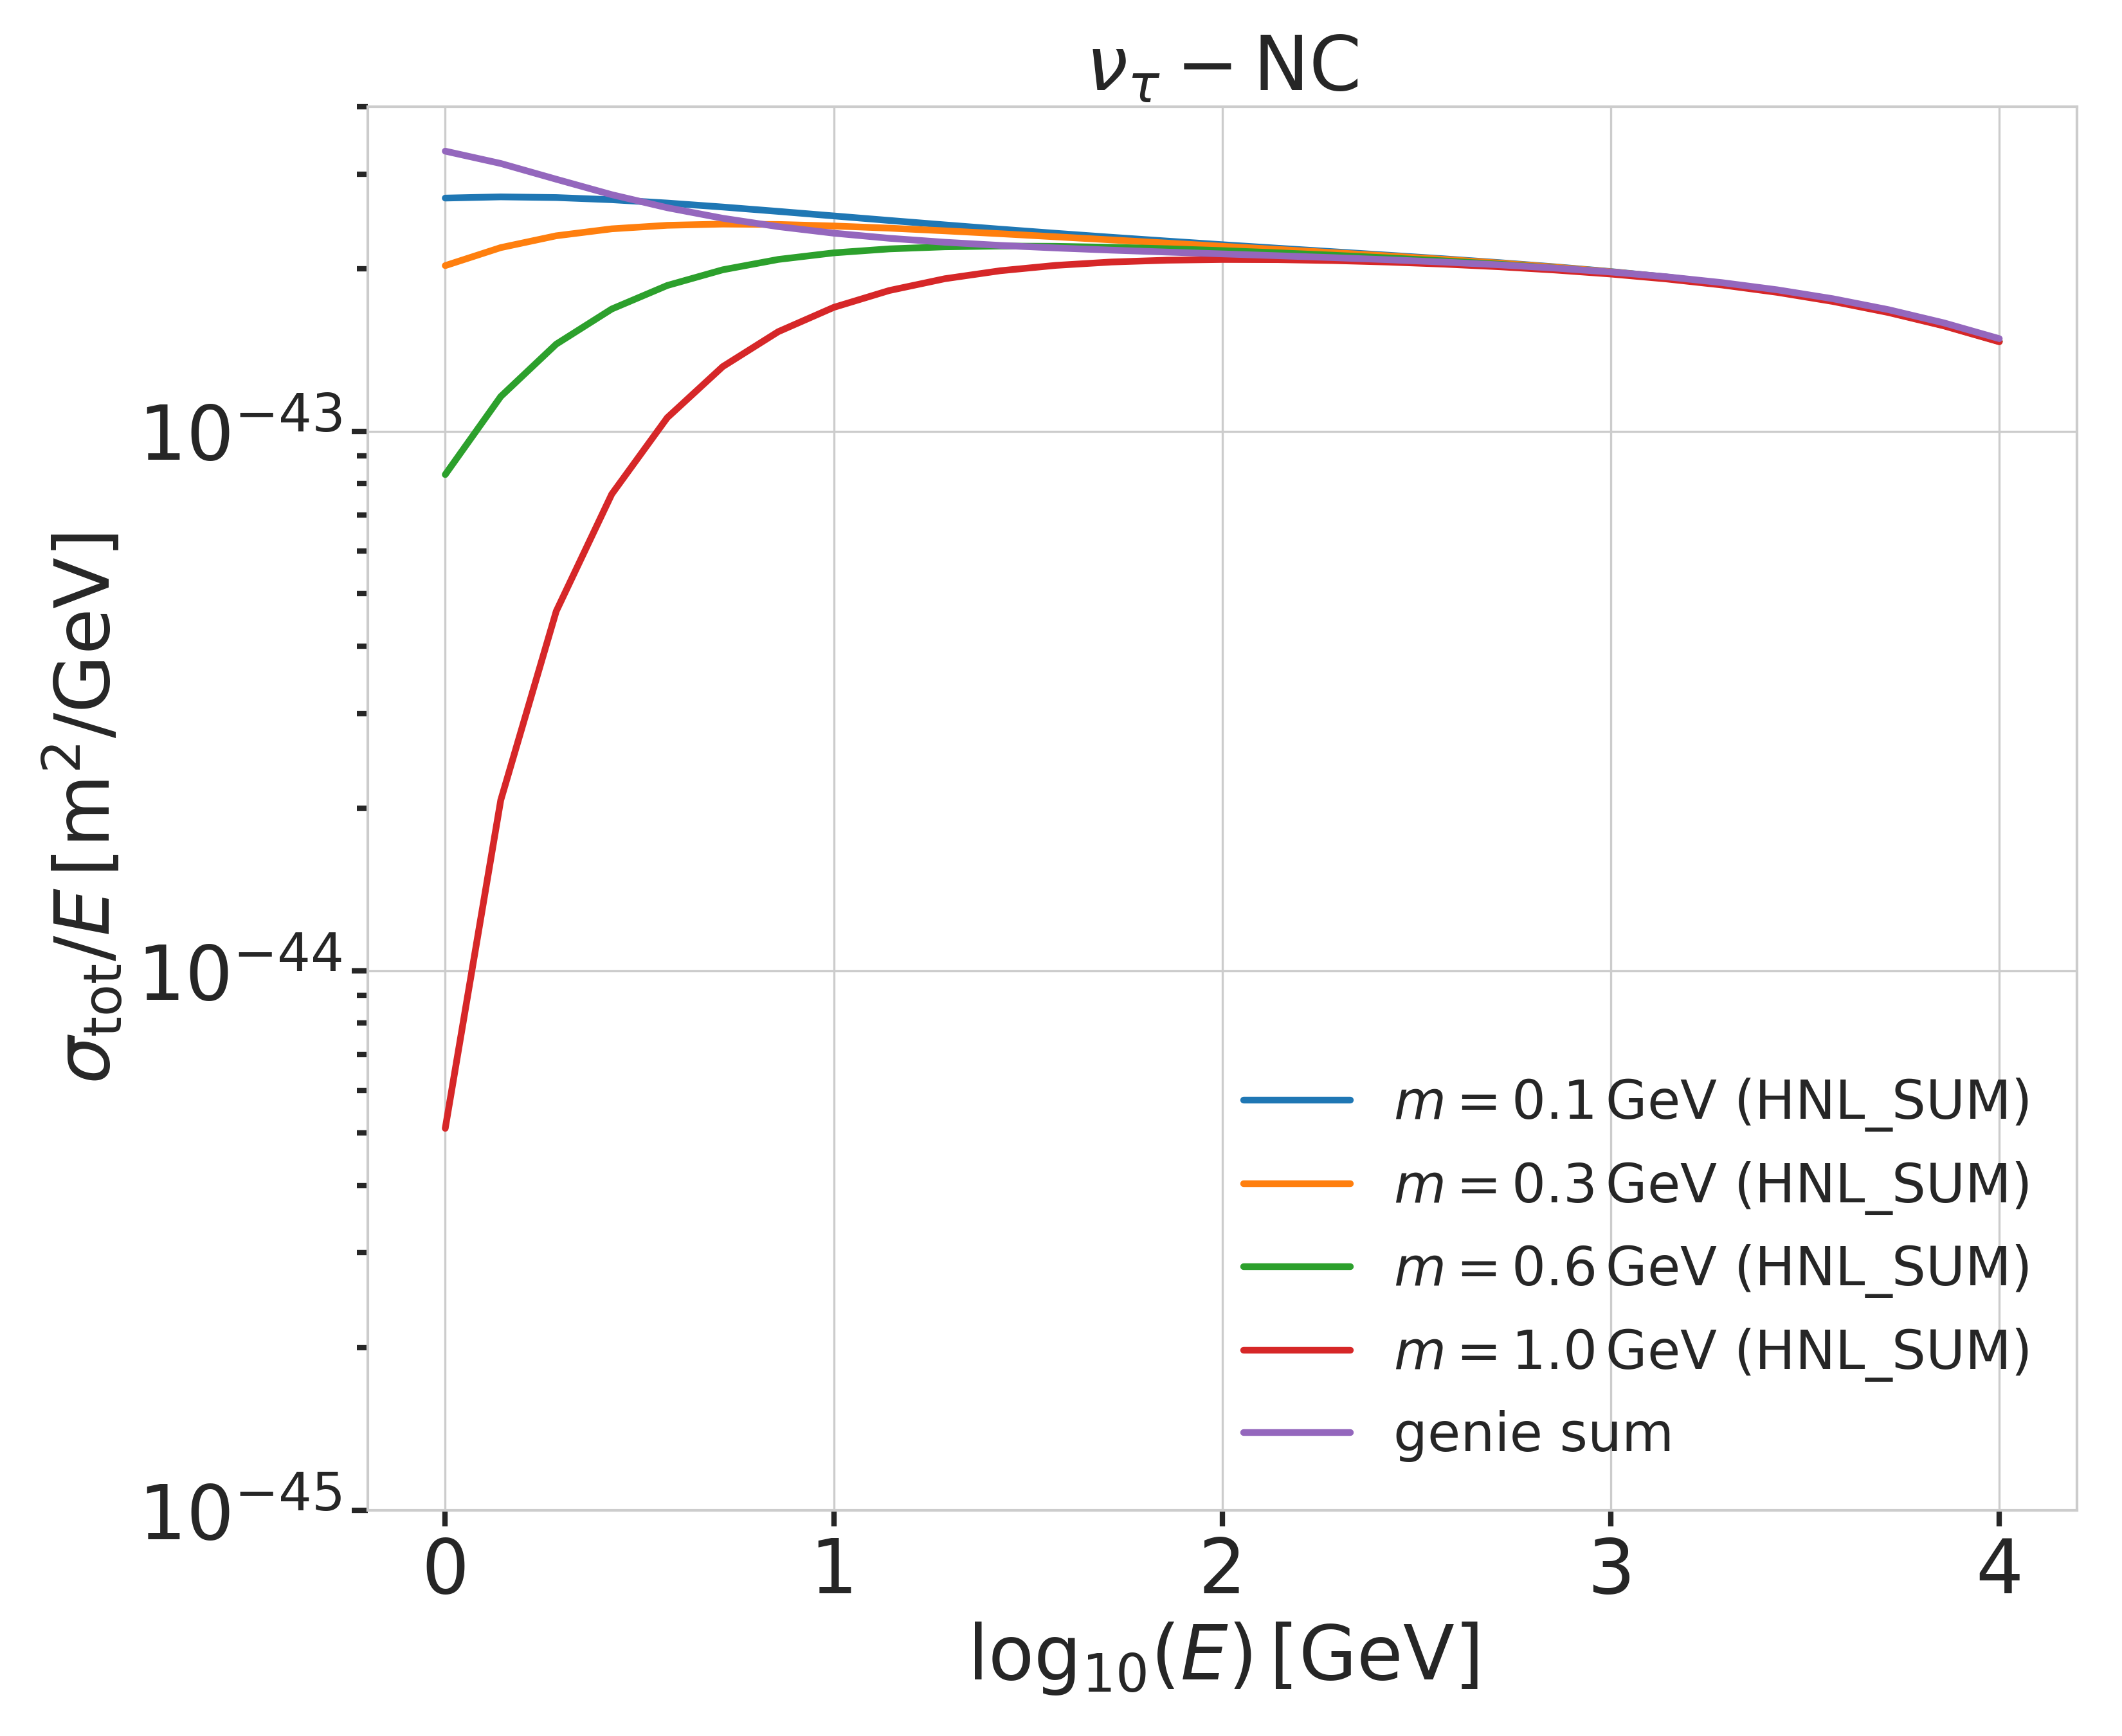
\includegraphics[width=.49\linewidth]{figures/hnl_simulation/cross_sections/custom_HNL_xsecs_final_SUM_flavorwise_total_xsecs_sigma-nutau-N-nc.png}
    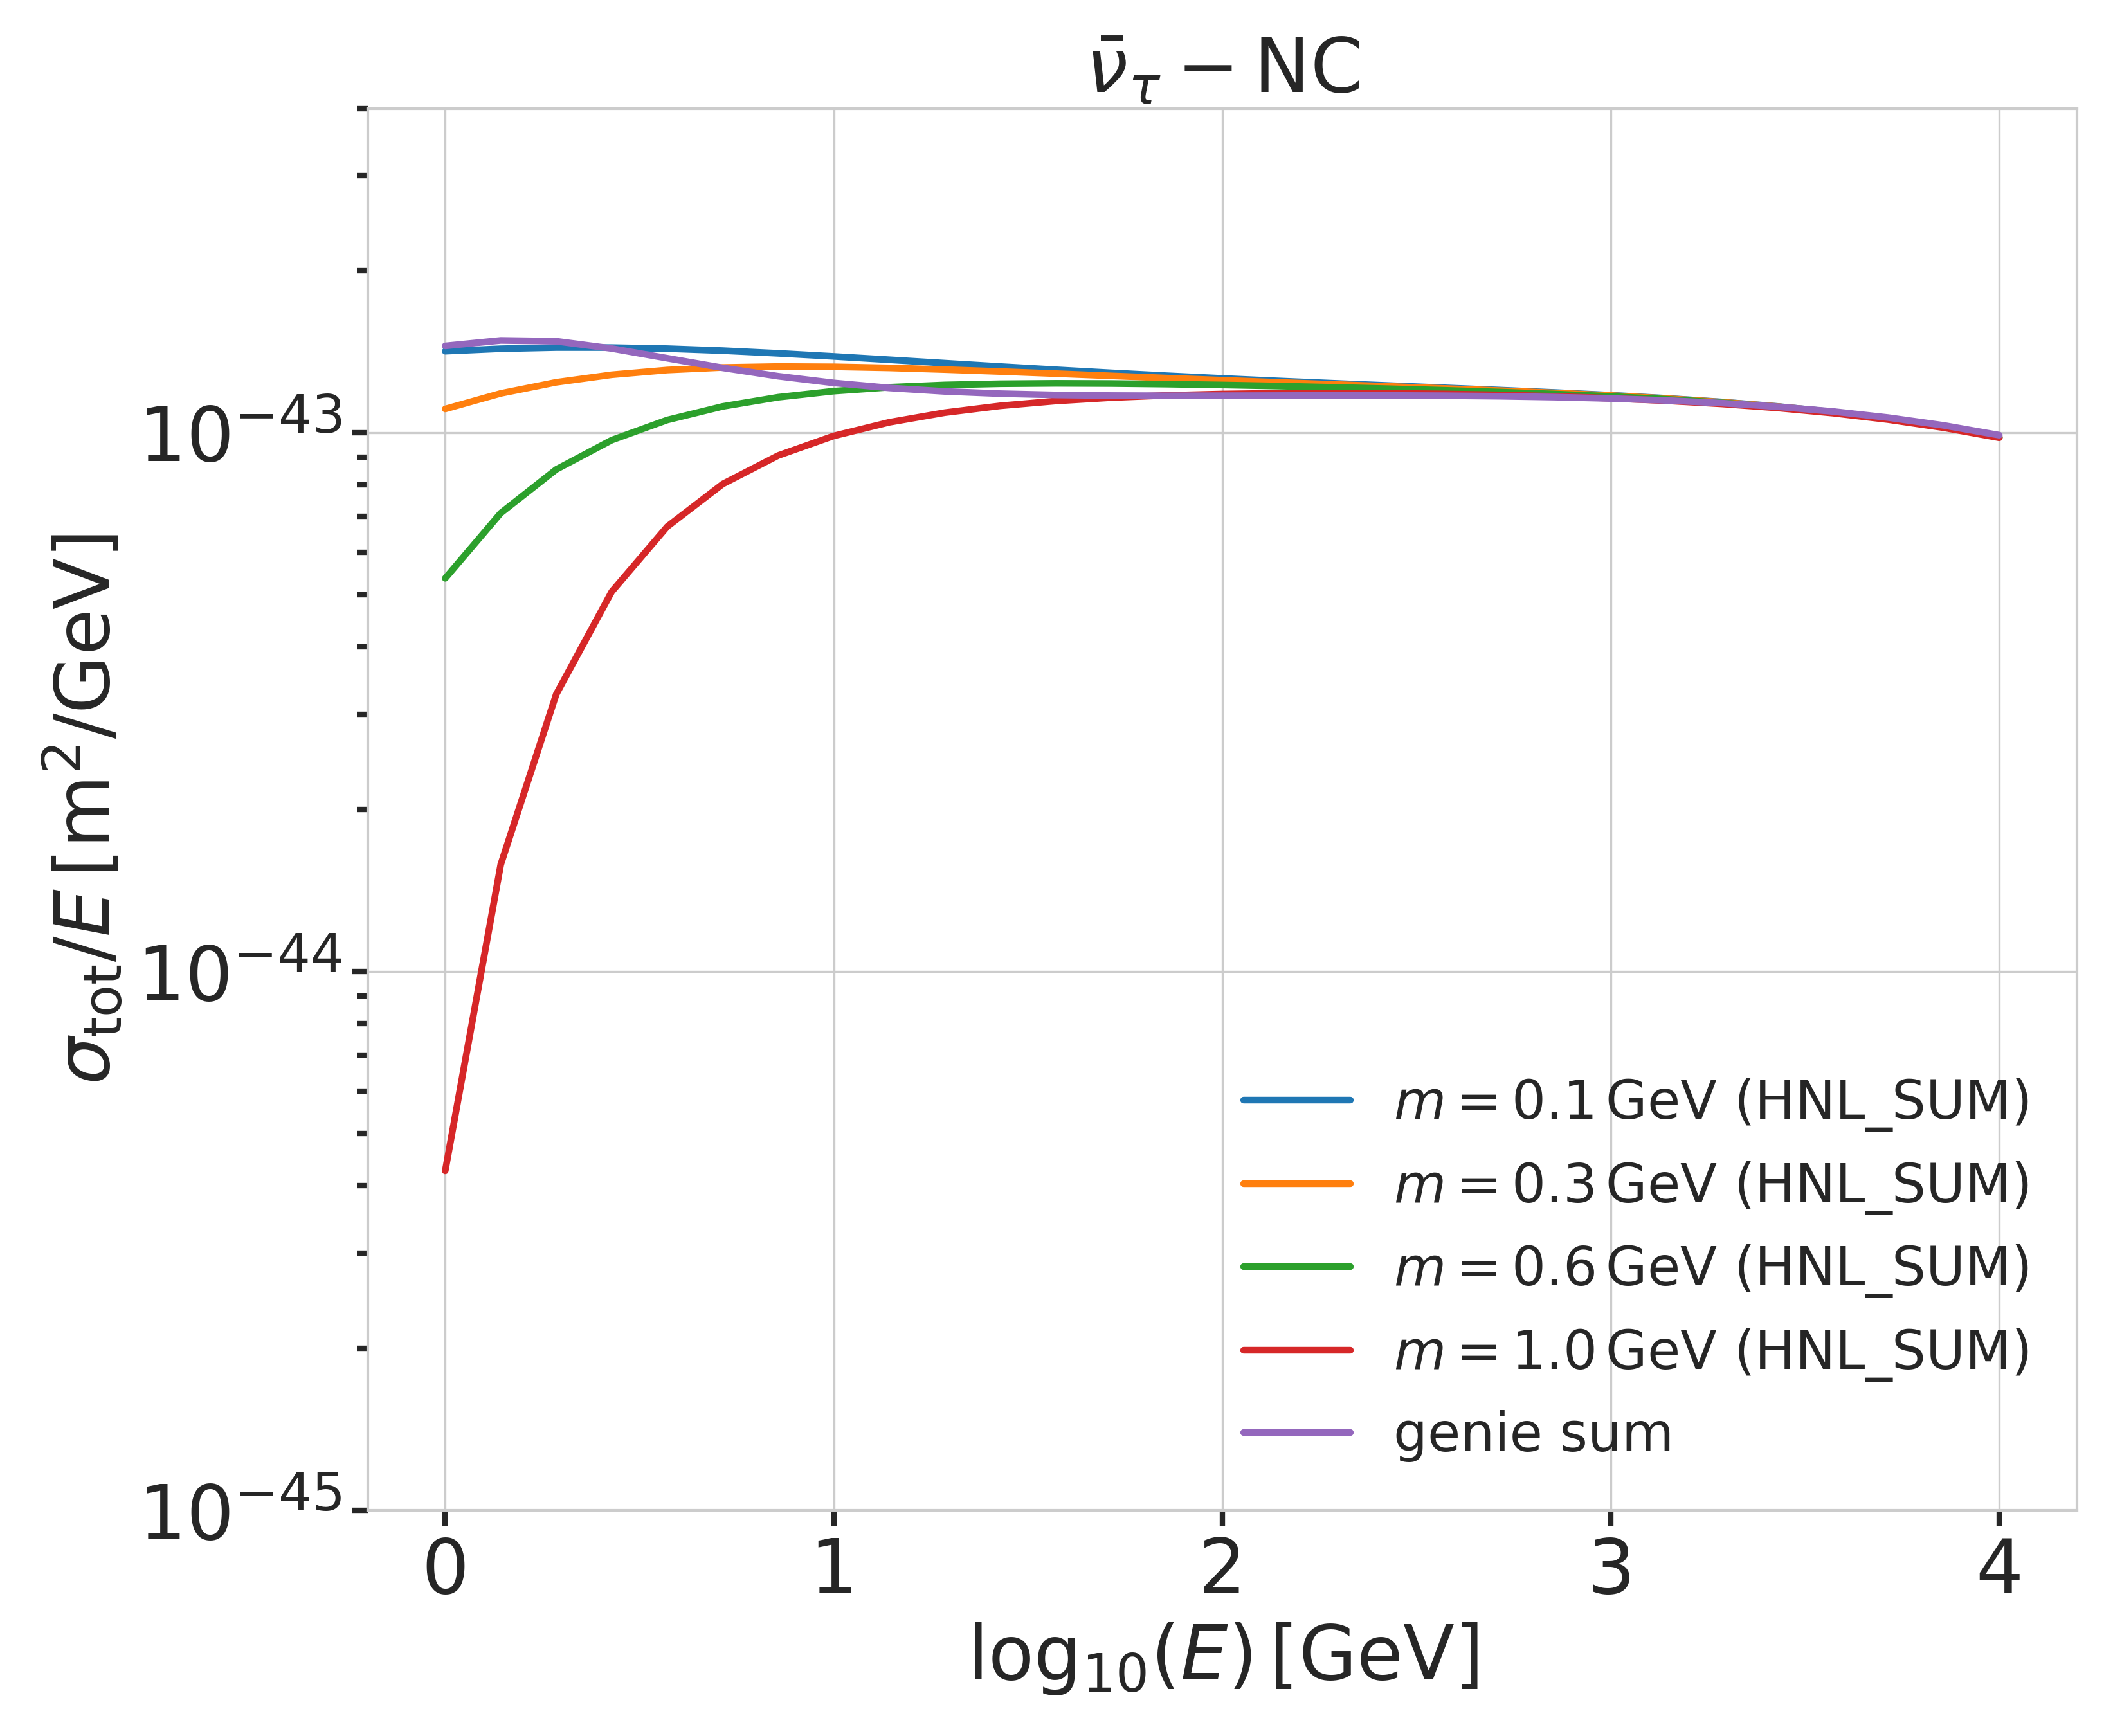
\includegraphics[width=.49\linewidth]{figures/hnl_simulation/cross_sections/custom_HNL_xsecs_final_SUM_flavorwise_total_xsecs_sigma-nutaubar-N-nc.png}
    \caption{Custom HNL total cross-sections for the four target masses compared to the total ($\nu_\tau$/$\bar{\nu}_\tau$ NC) cross-section used for SM neutrino simulation production with GENIE.}
    \labfig{custom_hnl_cross_sections}
\end{figure*}
\todo{Re-make plot with 3 target masses and better labels/legends etc.}

The GRV98LO PDFs were added to the cross-section spline maker and used to create the HNL cross-sections for consistency with the SM neutrino simulation that will be explained in \refsec{neutrino_generation}. The double-differential ($\rm{d}\sigma\rm{d}x\rm{d}y$) and total ($\sigma$) cross-sections were produced for the chosen target HNL masses and then splined in energy, $x$, and $y$ and just in the energy, respectively. The produced cross-section are added to the custom LI version and used for the simulation generation and weighting. \reffig{custom_hnl_cross_sections} shows the total cross-sections that were produced compared to the cross-section used for the production of the SM $\nu_\tau/\bar{\nu}_\tau$ NC background simulation. They agree above a certain energy ($\sim\SI{200}{\GeV}$), where the modification should not have any effect on the cross-sections, which is the desired result of using the identical input PDFs and confirms that the unmodified cross-sections produced with NuXSSplMkr agree with the GENIE cross-sections, which were used to generate the SM background MC.

\todo{SB:
emphasize the cut-off/suppression
}
\todo{Add comparisons of SM cross-sections between NuXSSplMkr and genie?}
\todo{add varied total cross-section for a few background HNL events (for QE/RES variations?!)}


\subsubsection{Decay Channels} \labsec{hnl_decay_channels}

The accessible decay channels are dependent on the mass of the HNL and the allowed mixing. For this analysis, where only $|U_{\tau4}|^2 \neq 0$, the decay channels considered are listed in \reftab{hnl_decay_channels} and the corresponding branching ratios are shown in \reffig{hnl_branching_ratios}. The individual branching ratio for a specific mass is calculated as $\mathrm{BR}_i(m_4)=\Gamma_i(m_4)/\Gamma_\mathrm{total}(m_4)$, where $\Gamma_\mathrm{total}(m_4)=\sum\Gamma_i(m_4)$.
% The formulas to calculate the decay widths show up in multiple references, but we chose to match them to \sidecite{Coloma:2020lgy}, which also discusses the discrepancies in previous literature.
The individual decay widths $\Gamma_i$ are computed using the state-of-the-art calculations from \sidecite{Coloma:2020lgy}, which are described in the following.

\begin{margintable}
    \footnotesize
    \begin{tabular} { lll }
        \hline\hline 
        \textbf{Channel} & \textbf{Opens} & \textbf{$\hat{\mathrm BR}$} \\
        \hline\hline 
        $\nu_4 \rightarrow \nu_\tau \nu_\alpha \bar{\nu_\alpha}$ & \SI{0}{\MeV} & 1.0 \\
        $\nu_4 \rightarrow \nu_\tau e^+ e^-$ & \SI{1}{\MeV} & ? \\
        $\nu_4 \rightarrow \nu_\tau \pi^0$ & \SI{135}{\MeV} & ? \\
        $\nu_4 \rightarrow \nu_\tau \mu^+ \mu^-$ & \SI{211}{\MeV} & ? \\
        $\nu_4 \rightarrow \nu_\tau \eta$ & \SI{548}{\MeV} & ? \\
        $\nu_4 \rightarrow \nu_\tau \rho^0$ & \SI{770}{\MeV} & ? \\
        $\nu_4 \rightarrow \nu_\tau \omega$ & \SI{783}{\MeV} & ? \\
        $\nu_4 \rightarrow \nu_\tau \eta'$ & \SI{958}{\MeV} & ? \\
        \hline
    \end{tabular}
    \caption[HNL mass dependent decay channels]{Possible decay channels of the HNL, considering only $|U_{\tau4}|^2 \neq 0$. Listed is the mass at which each channel opens and the maximum branching ratio.}
    \labtab{hnl_decay_channels}
\end{margintable}
\todo{Calculate max BRs}


\paragraph{2-Body Decay Widths}

The decay to a neutral pseudoscalar meson is
\begin{equation}
    \Gamma_{\nu_4 \rightarrow \nu_\tau P} = |U_{\tau4}|^2 \frac{G_F^2 m_4^3}{32\pi} f_P^2 (1-x_p^2)^2
    \;,
    \labeq{gamma_nu_P}
\end{equation}
with $x_P = m_P/m_4$ and the \textit{effective decay constants $f_P$} given by
% \begin{equation}
%     f_{\pi^0} = \SI{0.130}{\GeV}, \hspace{1cm} f_{\eta} = \SI{0.0816}{\GeV}, \hspace{1cm} f_{\eta'} = \SI{-0.0946}{\GeV}
%     \;,
%     \labeq{gamma_nu_P_f_factors}
% \end{equation}
\begin{align}
    f_{\pi^0} ={}& +\SI{0.1300}{\GeV}\;, \\
    f_{\eta} ={}& +\SI{0.0816}{\GeV}\;, \rm{and} \\
    f_{\eta'} ={}& -\SI{0.0946}{\GeV}\;,
    \labeq{gamma_nu_P_f_factors}
\end{align}
while the decay to a neutral vector meson is given by
\begin{equation}
    \Gamma_{\nu_4 \rightarrow \nu_\tau V} = |U_{\tau4}|^2 \frac{G_F^2 m_4^3}{32\pi} \bigg(\frac{f_V}{m_V}\bigg)^2 g_V^2 (1+2x_V^2) (1-x_V^2)^2
    \;,
    \labeq{gamma_nu_V}
\end{equation}
with $x_V = m_V/m_4$,
% \begin{equation}
%     f_{\rho^0} = \SI{0.171}{\square\GeV}, \hspace{1cm} f_{\omega} = \SI{0.155}{\square\GeV}
%     \;,
%     \labeq{gamma_nu_V_f_factors}
% \end{equation}
\begin{align}
    f_{\rho^0} ={}& \SI{0.171}{\square\GeV}\;, \\
    f_{\omega} ={}& \SI{0.155}{\square\GeV}\;,
    \labeq{gamma_nu_V_f_factors}
\end{align}
and
% \begin{equation}
%     g_{\rho^0} = 1-2\sin^2{\theta_w}, \hspace{1cm} g_{\omega} = \frac{-2\sin^2{\theta_w}}{3}, \hspace{1cm} \sin^2{\theta_w} = 0.2229
%     \labeq{gamma_nu_V_g_factors}
% \end{equation}
\begin{align}
    g_{\rho^0} ={}& 1-2\sin^2{\theta_w}\;, \\
    g_{\omega} ={}& \frac{-2\sin^2{\theta_w}}{3}\;,
    \labeq{gamma_nu_V_g_factors}
\end{align}
and $\sin^2{\theta_w}=0.2229$ \sidecite{codata2018}, where $\theta_w$ is the Weinberg angle.


\paragraph{3-Body Decay Widths}

The (invisible) decay to three neutrinos, one of flavor $\tau$ and two of any flavor $\alpha$, is
\begin{equation}
    \Gamma_{\nu_4 \rightarrow \nu_\tau \nu_\alpha \bar{\nu_\alpha}} = |U_{\tau4}|^2 \frac{G_F^2 m_4^5}{192\pi^3}
    \;,
    \labeq{gamma_nu_nu_nu}
\end{equation}
while the decay to two charged leptons (using $x_\alpha = (m_\alpha/m_4)^2)$ of the same flavor reads
\begin{equation}
    \Gamma_{\nu_4 \rightarrow \nu_\tau l_\alpha^+ l_\alpha^-} = |U_{\tau4}|^2 \frac{G_F^2 m_4^5}{192\pi^3} \big[ C_1 f_1(x_\alpha) + C_2 f_2(x_\alpha) \big]
    \;,
    \labeq{gamma_nu_ll_full}
\end{equation}
with the constants defined as
% \begin{equation}
%     C_1 = \frac{1}{4}(1-4\sin^2{\theta_w}+8\sin^4{\theta_w}) , \hspace{1cm} C_2 = \frac{1}{2}(-\sin^2{\theta_w}+2\sin^4{\theta_w})
%     \;,
%     \labeq{gamma_nu_ll_c1_c2}
% \end{equation}
\begin{align}
    C_1 ={}& \frac{1}{4}(1-4\sin^2{\theta_w}+8\sin^4{\theta_w})\;, \\
    C_2 ={}& \frac{1}{2}(-\sin^2{\theta_w}+2\sin^4{\theta_w})\;,
    \labeq{gamma_nu_ll_c1_c2}
\end{align} 
the functions as
\begin{equation}
    f_1(x_\alpha) = (1-14x_\alpha-2x_\alpha^2-12x_\alpha^3)\sqrt{1-4x_\alpha}+12x_\alpha^2(x_\alpha^2-1)L(x_\alpha)
    \;,
    \labeq{gamma_nu_ll_f1}
\end{equation}
\begin{equation}
    f_2(x_\alpha) = 4[x_\alpha(2+10x_\alpha-12x_\alpha^2)\sqrt{1-4x_\alpha}+6x_\alpha^2(1-2x_\alpha+2x_\alpha^2)L(x_\alpha)]
    \;,
    \labeq{gamma_nu_ll_f2}
\end{equation}
and
\begin{equation}
    L(x) = \ln \biggl( \frac{ 1-3x_\alpha-(1-x_\alpha)\sqrt{1-4x_\alpha} }{ x_\alpha(1+\sqrt{1-4x_\alpha}) } \biggr)
    \;.
    \labeq{gamma_nu_ll_l}
\end{equation}


% \subsubsection{2-Body Decay Kinematics} \labsec{2body_decay_kinematics}
\todo{JVS:
consider also writing down the (trivial) 2-body decay kinematics for completeness and consistency. This transition is a bit jarring as it is
}

\subsubsection{3-Body Decay Kinematics with MadGraph} \labsec{madgraph_3body_decays}

The specific MadGraph version used to produce the 3-body decay kinematics is \textsc{MadGraph4 v3.4.0} \cite{madgraph4}, which uses the decay diagrams calculated with \textsc{FeynRules 2.0} \sidecite{feynrules2} and the Lagrangians derived in \sidecite{Coloma:2020lgy} as input. The \textit{Universal FeynRules Output (UFO)} from \textsc{effective\_HeavyN\_Majorana\_v103} were used for our calculation. For each mass and corresponding decay channels, we produce \SI{1e06}{} decay kinematic variations in the rest frame and store those in a text file. During event generation, we uniformly select an event from that list, to simulate the decay kinematics of a 3-body decay.


\subsection{Sampling Distributions} \labsec{hnl_sampling_distributions}

In principle, the generation level sampling distributions should be chosen such that at final level of the selection chain the phase space relevant for the analysis is covered with sufficient statistics to make a reasonable estimate of the event expectation. Initial distributions insufficiently covering the phase space leads to an underestimate of the expected rates, because part of the events that would pass the selection are not produced. This limits the expected analysis potential.
% This would still be correct as in being the more conservative estimate, but it would limit the analysis potential.
Three discrete simulation samples were produced with HNL masses of \SI{0.3}{\GeV}, \SI{0.6}{\GeV}, and \SI{1.0}{\GeV}. Because during development it became clear that the low lengths component is crucial to get a reasonable event estimate, each sample consists of a part that is generated for very short decay lengths and one for long decay lengths. The remaining sampling distributions are identical for all samples and are listed in \reftab{hnl_realistic_sample_sampling_distributions}. The target number of events for each sample was \SI{2.5e9}{}.

\begin{table}[h]
    \centering
    \begin{tabular} { lll }
        \hline \hline 
        \textbf{Variable} & \textbf{Distribution} & \textbf{Range/Value} \\
        \hline \hline 
        energy & $E^{-2}$ & [\SI{2}{\GeV}, \SI{1e4}{\GeV}] \\
        zenith & uniform (in $\cos(\theta)$) & [\SI{80}{\degree}, \SI{180}{\degree}] \\
        azimuth & uniform & [\SI{0}{\degree}, \SI{360}{\degree}] \\
        vertex $x,y$ & uniform & $r$=\SI{600}{\metre} \\
        vertex $z$ & uniform & \SIrange{-600}{0}{\metre} \\
        $m_\mathrm{4}$ & fixed & [0.3, 0.6, 1.0]\,\si{\GeV} \\
        $L_\mathrm{decay}$ & $L^{-1}$ & [0.0004, 1000]\,\si{\metre} \\
        \hline
    \end{tabular}
    \caption[Model dependent simulation sampling distributions]{Generation level sampling distributions and ranges/values of the model dependent simulation samples.}
    \labtab{hnl_realistic_sample_sampling_distributions}
\end{table}


\subsection{Weighting Scheme} \labsec{hnl_weighting_scheme}

\todo{JVS:
    The build-up of the weight expression is hard to follow without knowing where it’s going. It may be better to start with the fact that the importance sampling weight is the ratio of PDFs, then write down each pdf, then drill down into each of the terms (basically, the standard “tell me what you’re going to tell me, then tell me, then tell me what you told me” scheme).
}

To produce physically correct event distributions based on the simplified generation sampling distributions for the HNL simulation, the forward folding method that was already introduced for the SM simulation in \refsec{sm_event_generation} is also used. The weighting scheme that will be explained in the following is implemented in a custom stage\sidenote{An analysis in PISA is a collection of functions that are written in so-called \textit{stages}. The stages can be combined in a \textit{pipeline} and are executed in a specific order. This particular stage is located in \texttt{pisa$/$stages$/$aeff$/$weight\_hnl.py}.} in the IceCube low energy analysis framework PISA \cite{pisa_software} \sidecite{pisa_paper}, which will be discussed in \refsec{analysis_framework}.
% The custom weighting scheme is implemented in \href{https://github.com/icecube/pisa/blob/master/pisa/stages/aeff/weight_hnl.py}{this custom stage}.
The only required input is the mixing strength $|U_{\tau4}|^2$, which is the variable physics parameter in this analysis.
% This weighting is needed to go from the used decay length sampling distribution (inverse $1/L$ with fixed range in lab frame) to the target distribution (exponential defined by proper lifetime of the HNL).
For each event the gamma factor
\begin{equation}
    \gamma = \frac{\sqrt{E_\mathrm{kin}^2+m_4^2}}{m_4}
    \;,
    \labeq{gamma_factor}
\end{equation}
is calculated, with the HNL mass $m_4$, and its kinetic energy $E_\mathrm{kin}$. The speed of the HNL is calculated as
\begin{equation}
    v = c \cdot \sqrt{1 - \frac{1}{\gamma^2}}
    \;,
    \labeq{lorentz_speed}
\end{equation}
where $c$ is the speed of light. With these, the lab frame decay length range $[s_\mathrm{min},s_\mathrm{max}]$ can be converted into the rest frame lifetime range $[\tau_\mathrm{min},\tau_\mathrm{max}]$ for each event
\begin{equation}
    \tau_\mathrm{min/max} = \frac{s_\mathrm{min/max}}{v\cdot\gamma}.
\end{equation}
The proper lifetime of each HNL event can be calculated using the total decay width $\Gamma_\mathrm{total}$ from \refsec{hnl_decay_channels} and the chosen mixing strength $|U_{\tau4}|^2$ as
\begin{equation}
    \tau_\mathrm{proper} = \frac{\hbar}{\Gamma_\mathrm{total}(m_4) \cdot |U_{\tau4}|^2}
    \;,
    \labeq{proper_lifetime}
\end{equation}
where $\hbar$ is the reduced Planck constant. Since the decay lengths or lifetimes of the events are sampled from an inverse distribution instead of an exponential, as it would be expected from a particle decay, we have to re-weight accordingly to achieve the correct decay lengths or lifetimes distribution. This is done by using the wanted exponential distribution
\begin{equation}
    \mathrm{PDF}_\mathrm{exp} = \frac{1}{\tau_\mathrm{proper}} \cdot e^{\frac{-\tau}{\tau_\mathrm{proper}}}
    \;,
    \labeq{pdf_exponential}
\end{equation}
and the inverse distribution that was sampled from
\begin{equation}
    \mathrm{PDF}_\mathrm{inv} = \frac{1}{\tau \cdot (\ln(\tau_\mathrm{max}) - \ln(\tau_\mathrm{min}))}
    \;.
    \labeq{pdf_inverse}
\end{equation}
This re-weighting factor is then calculated as
\begin{equation}
    w_\mathrm{lifetime} = \frac{\mathrm{PDF}_\mathrm{exp}}{\mathrm{PDF}_\mathrm{inv}} = \frac{\Gamma_\mathrm{total}(m_4) \cdot |U_{\tau4}|^2}{\hbar} \cdot \tau \cdot (\ln(\tau_\mathrm{max}) - \ln(\tau_\mathrm{min})) \cdot e^{\frac{-\tau}{\tau_\mathrm{proper}}}
    \;.
    \labeq{weight_lifetime}
\end{equation}
Adding another factor of $|U_{\tau4}|^2$ to account for the mixing at the interaction vertex the total re-weighting factor becomes
\begin{equation}
    w_\mathrm{total} = |U_{\tau4}|^2 \cdot w_\mathrm{lifetime}
    \;.
    \labeq{weight_full}
\end{equation}
If this additional weighting factor is multiplied to a generation weight with units \si{\meter^2} (like in \refeq{neutrino_generation_weight}), the livetime in \si{\second}, and the oscillated primary neutrino flux in \si{\meter^{-2}\second^{-1}}, it results in the number of expected events in the detector for this particular MC event for a chosen mixing (and mass).

\todo{add table with number of gen level files? mention the event number is smaller because of kinemtic condition?}

\subsection{Generation Level Distributions}

\reffig{hnl_gen_distris} shows some selected generation level distributions. Additional distributions can be found in \reffig{hnl_gen_distris_appendix}.

\todo{Combine low/high plots and remove all traces of the separation in the thesis (tables/text/etc.)}

\begin{figure*}[h]
    \centering
    \begin{subfigure}{0.49\linewidth}
        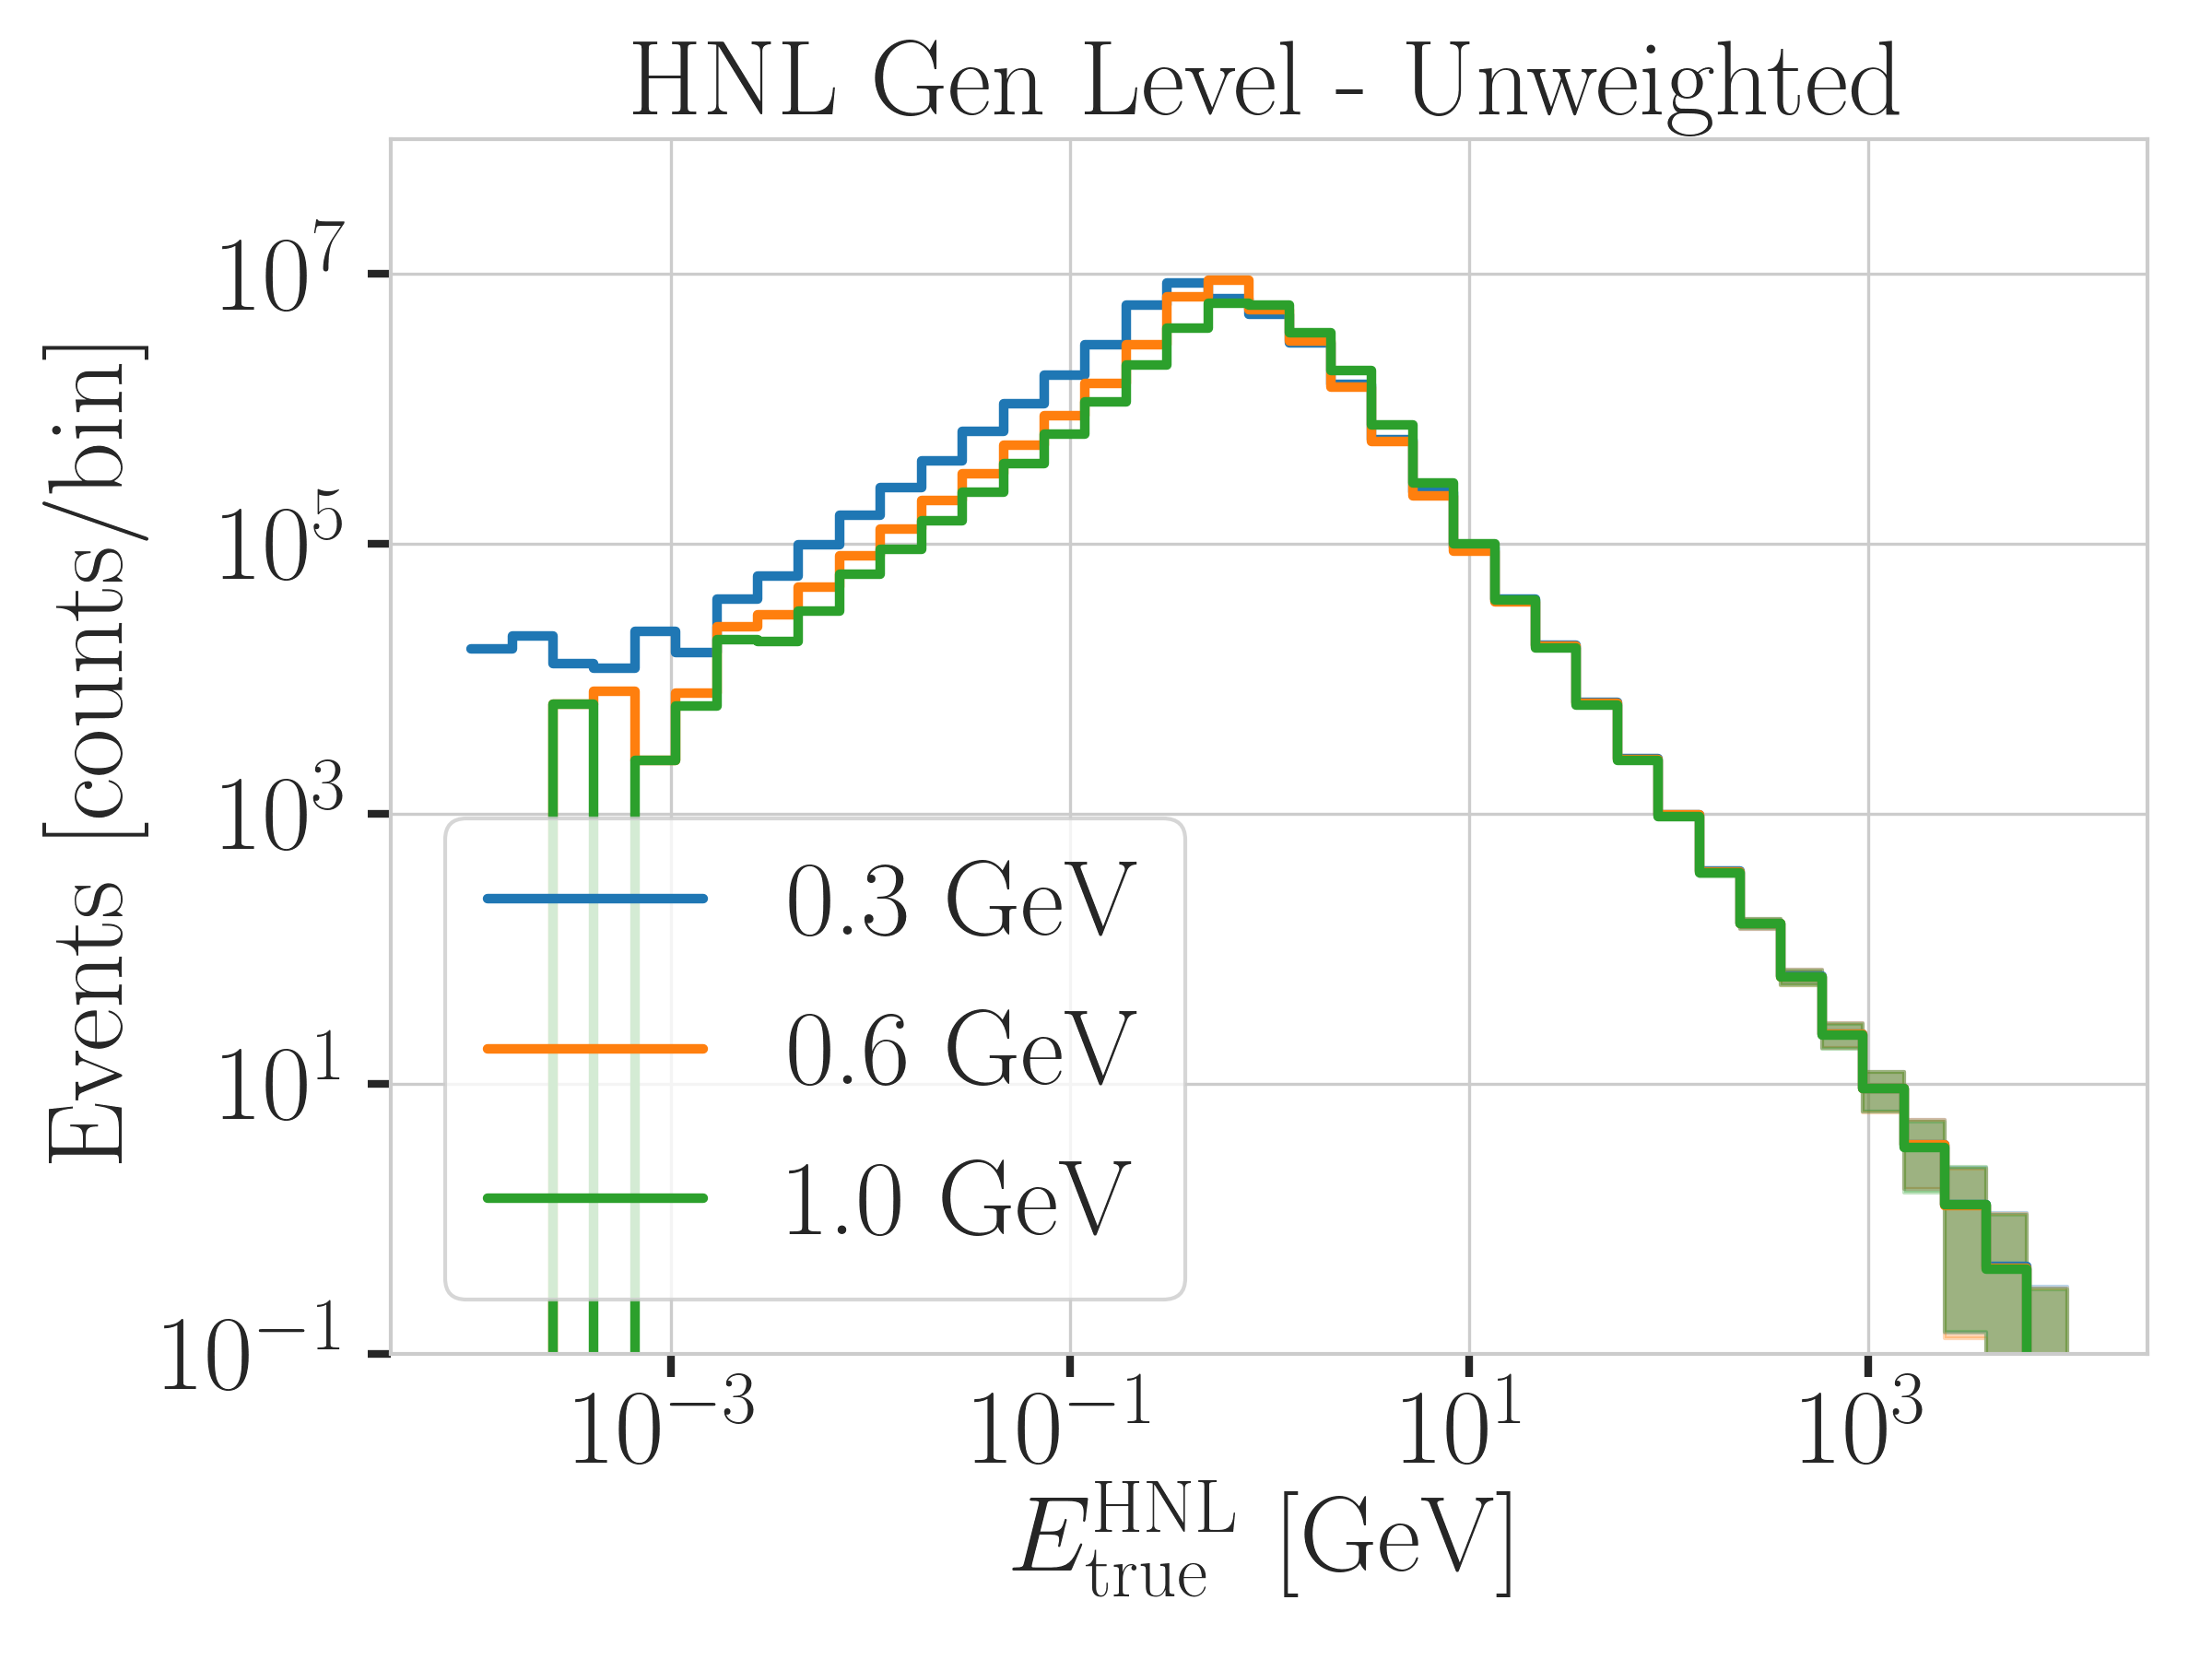
\includegraphics{figures/hnl_simulation/generation/1_d_distr_HNL_true_energy_gen_level_unweighted.png}
        \caption{HNL energy}
    \end{subfigure}
    \begin{subfigure}{0.49\linewidth}
        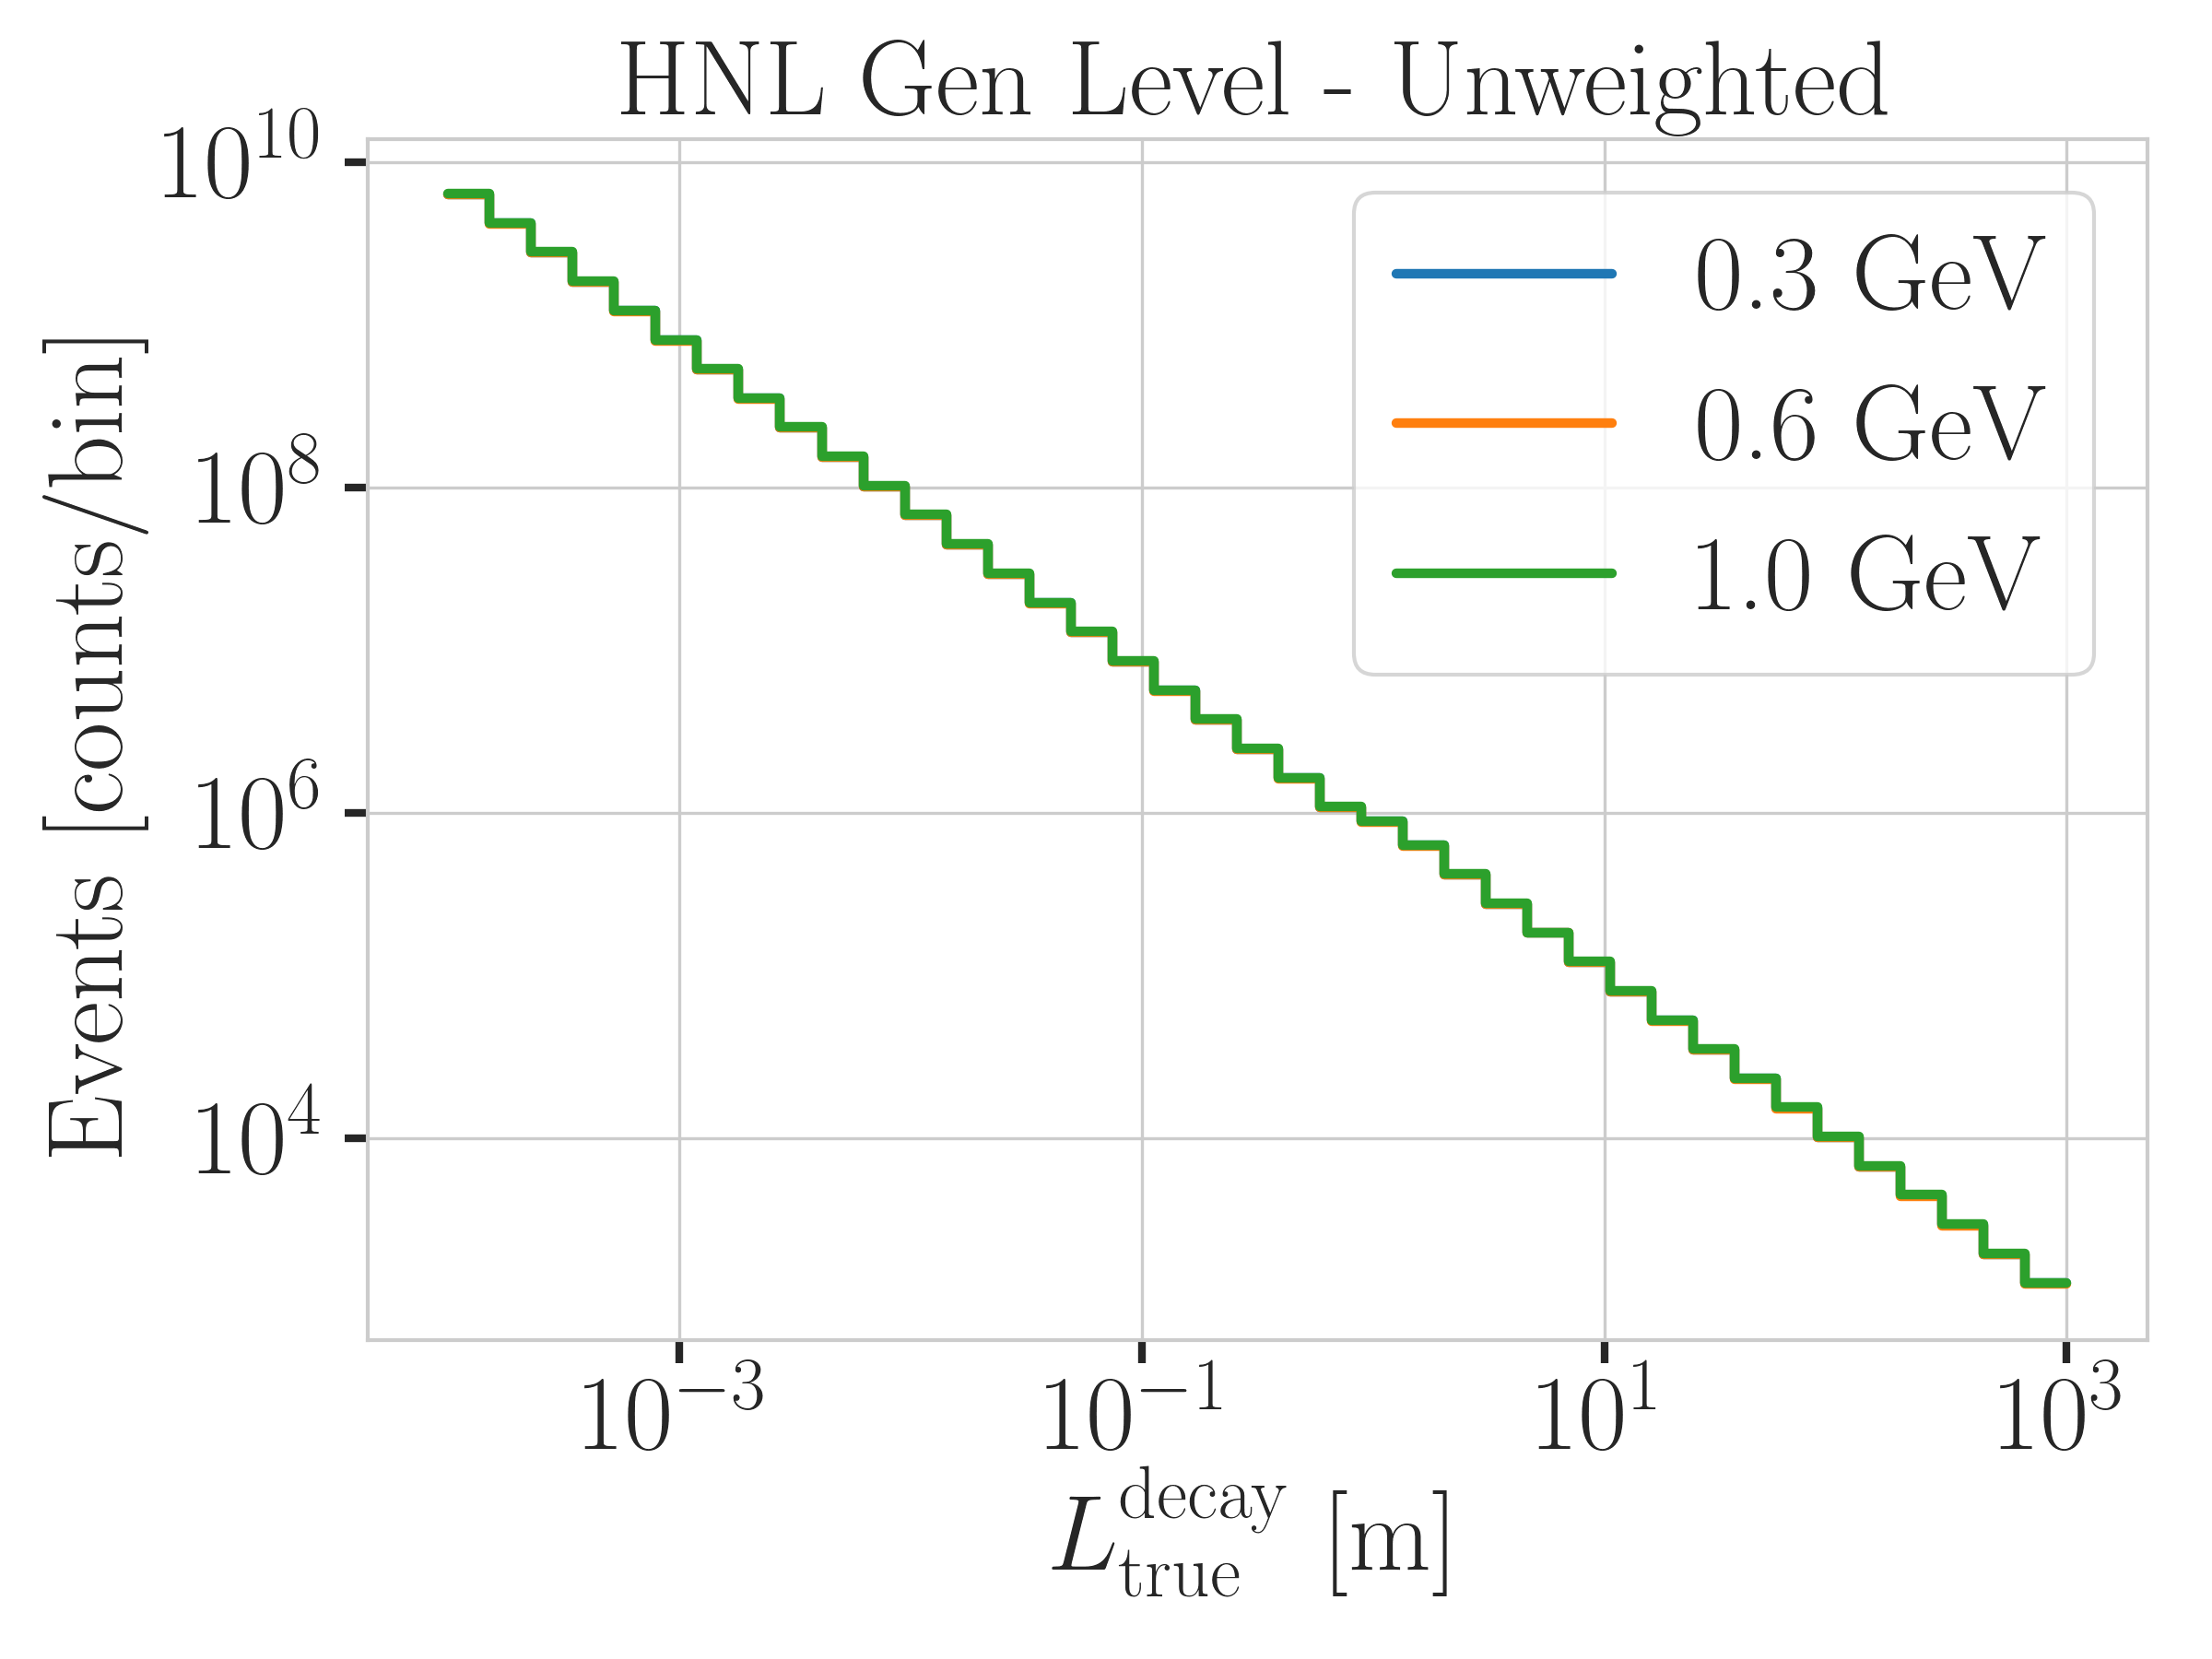
\includegraphics{figures/hnl_simulation/generation/1_d_distr_distance_gen_level_unweighted.png}
        \caption{Decay length}
    \end{subfigure}
    \begin{subfigure}{0.49\linewidth}
        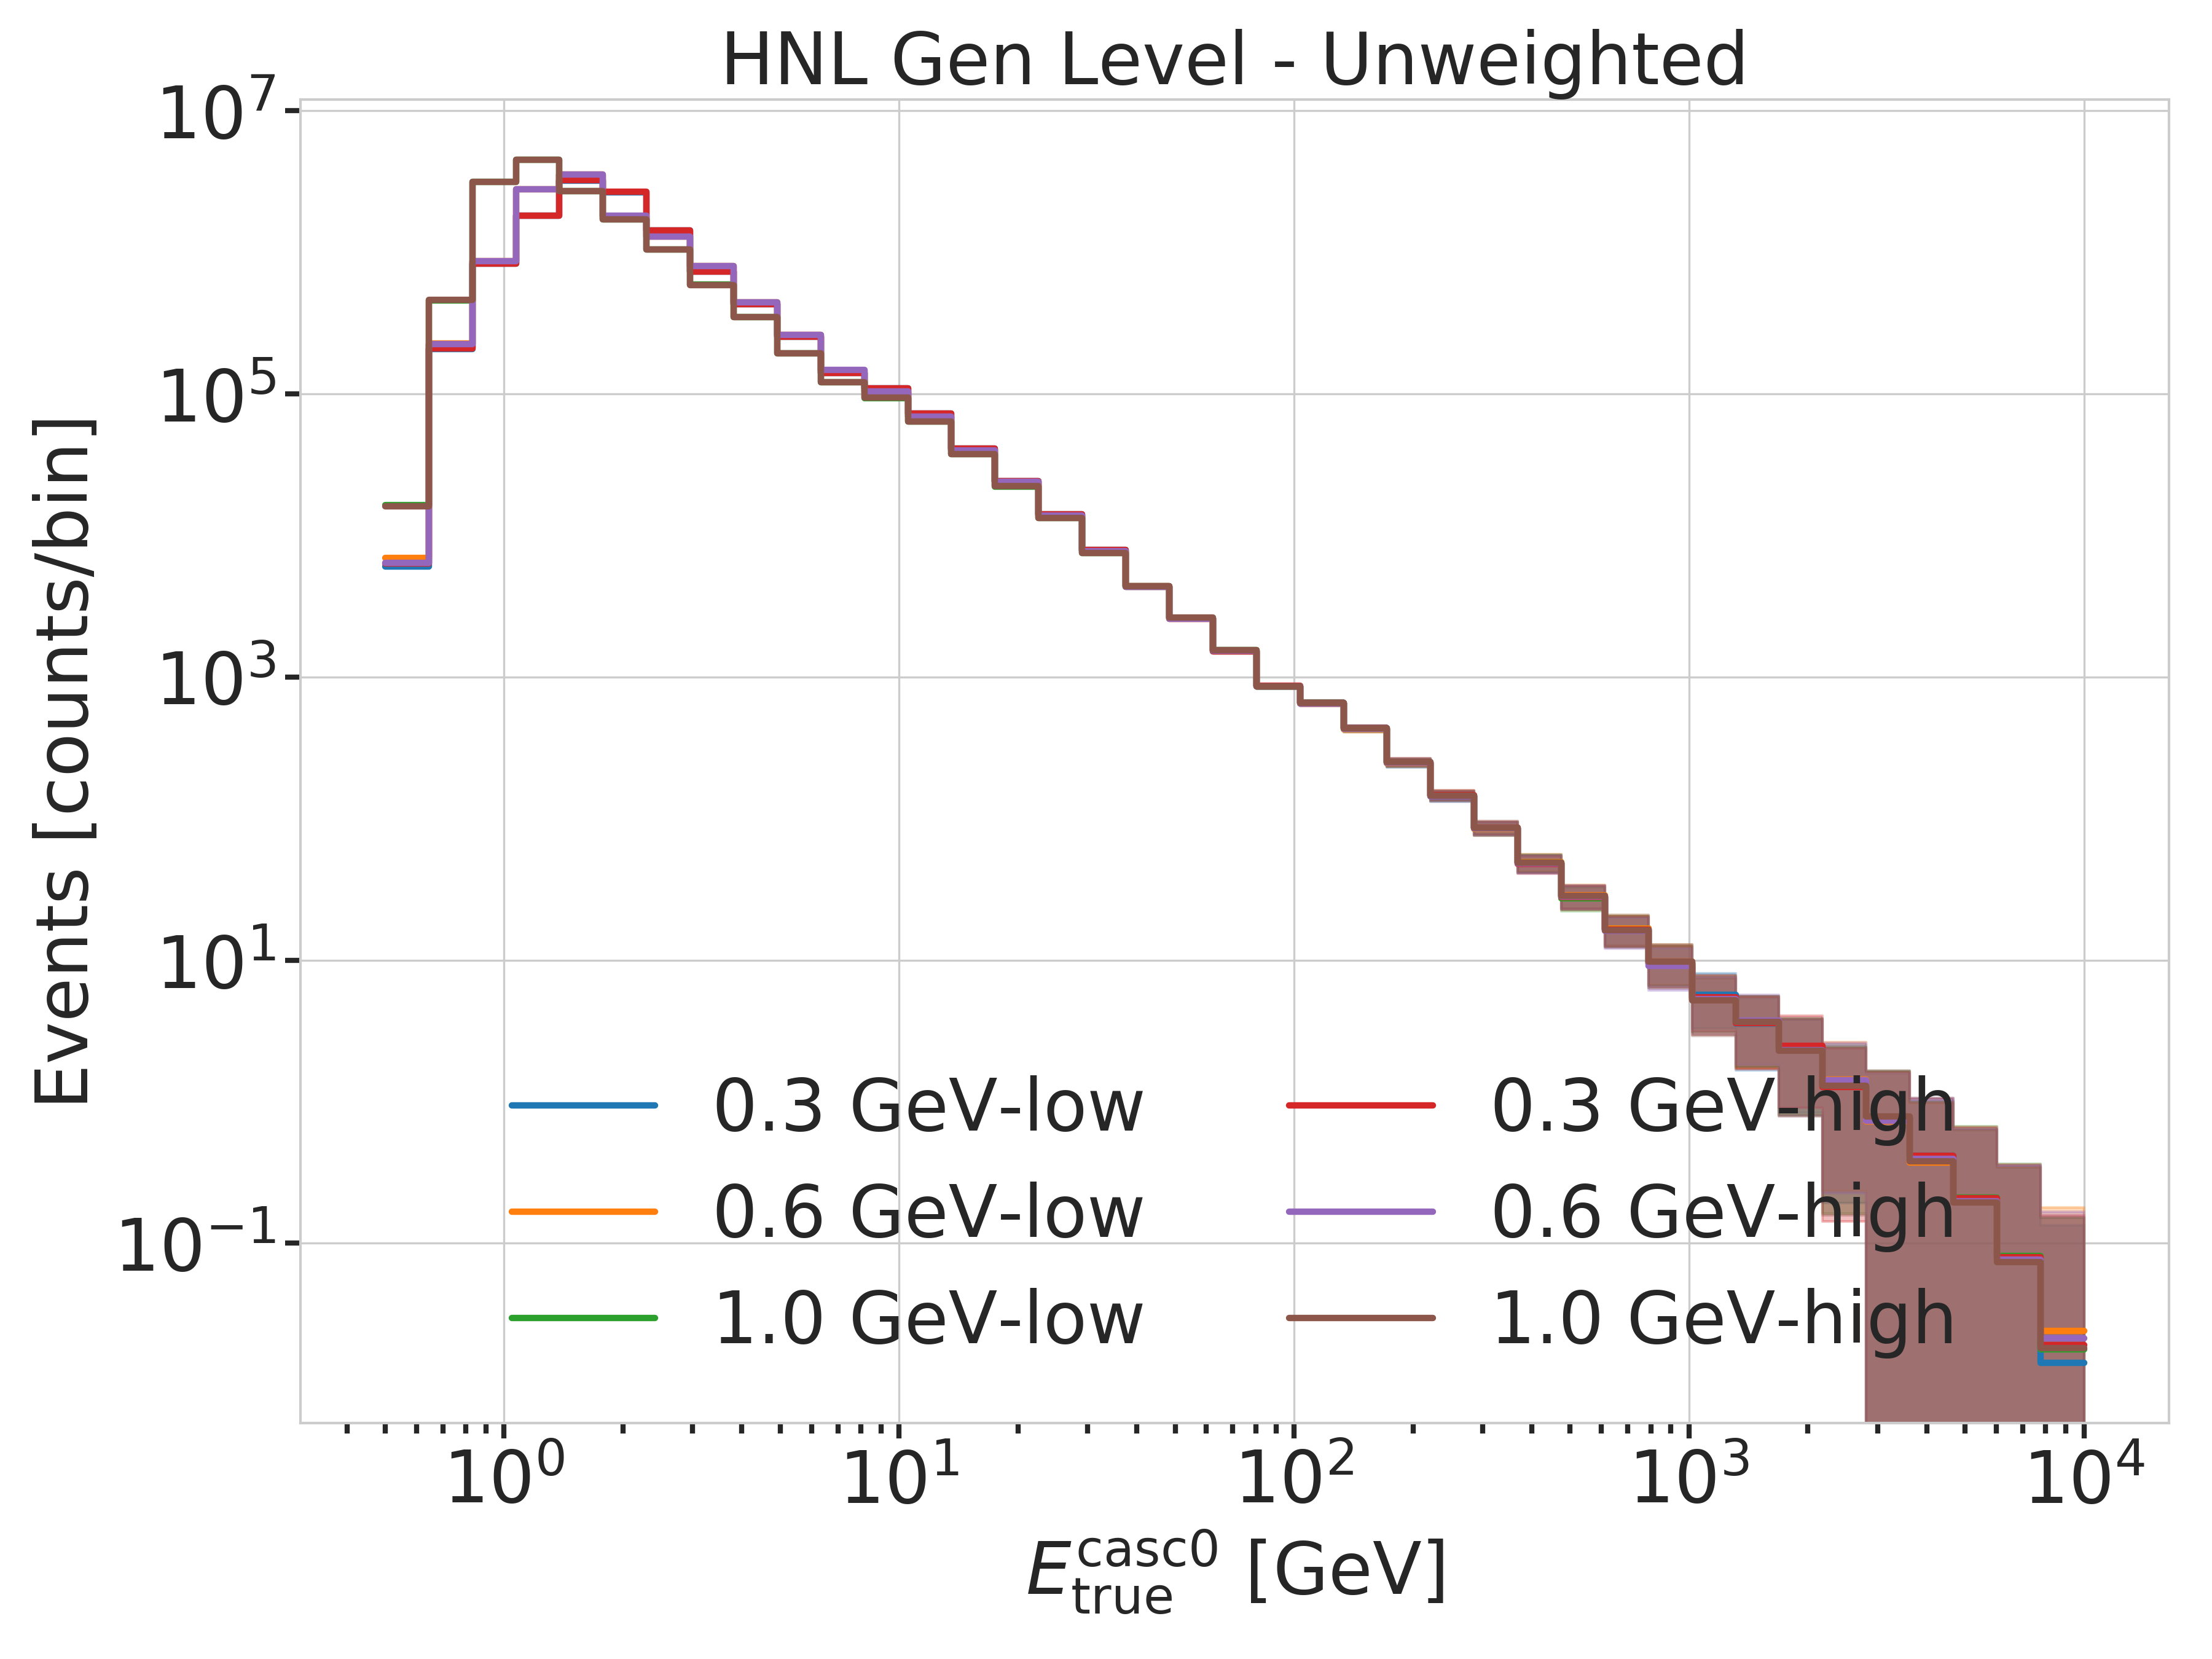
\includegraphics{figures/hnl_simulation/generation/1_d_distr_casc0_true_energy_gen_level_unweighted.png}
        \caption{First cascade energy}
    \end{subfigure}
    \begin{subfigure}{0.49\linewidth}
        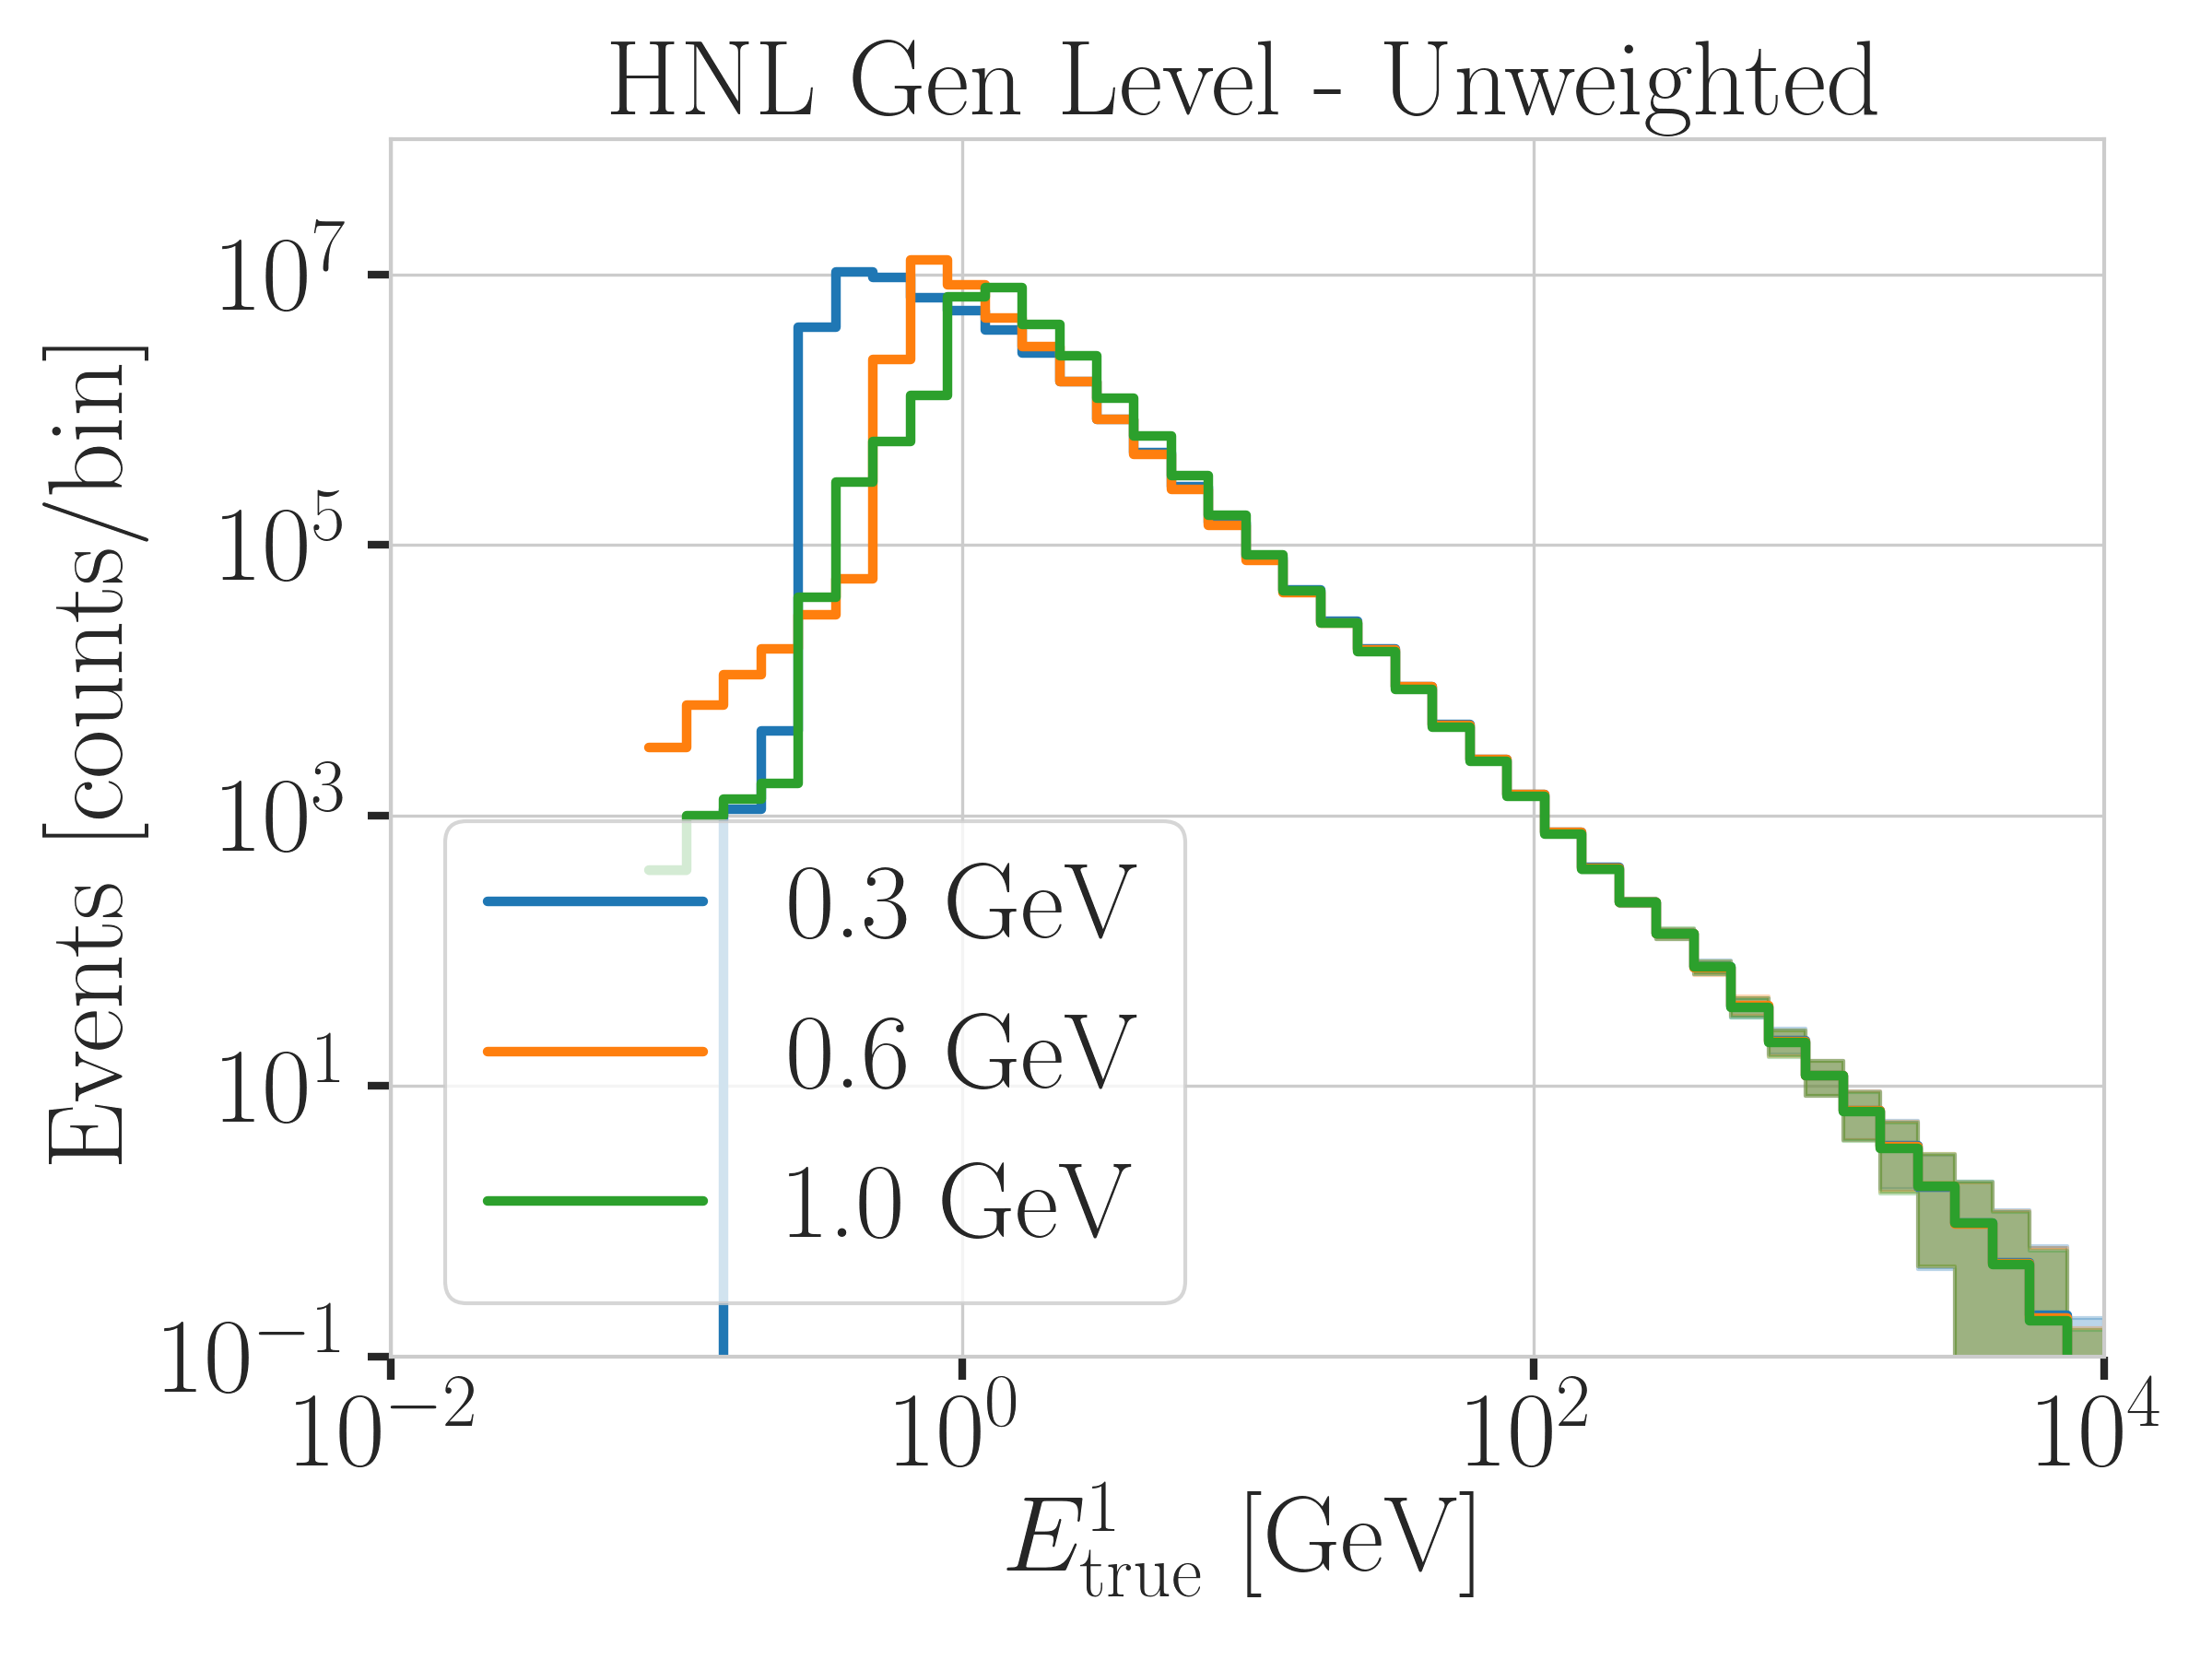
\includegraphics{figures/hnl_simulation/generation/1_d_distr_casc1_true_energy_gen_level_unweighted.png}
        \caption{Second cascade energy}
    \end{subfigure}
    \caption[Model dependent simulation generation level distributions]{Generation level distributions of the model dependent simulation.}
    \labfig{hnl_gen_distris}
\end{figure*}

\todo{What is the message of these plots? Make it clear in the text and also in the captions. Potentially cut down to one or two and leave the rest or move them to the appendix.}
